
\documentclass[8pt,landscape]{extarticle}
\usepackage{amssymb,amsmath,amsthm,amsfonts}
\usepackage{multicol,multirow}
\usepackage{calc}
\usepackage{ifthen}
\usepackage[landscape]{geometry}
\usepackage[colorlinks=true,citecolor=blue,linkcolor=blue]{hyperref}
\usepackage{graphicx}
\usepackage{commath}
\usepackage{listings}
\usepackage{microtype}
\usepackage[compact,small]{titlesec}
\usepackage{enumitem}
\setlist[itemize]{nosep, topsep=0pt}
\setenumerate{nosep,topsep=0pt,parsep=0pt,partopsep=0pt}
\graphicspath{ {./images/} }
\ifthenelse{\lengthtest { \paperwidth = 11in}}
    { \geometry{top=.5cm,left=.5cm,right=.5cm,bottom=.5cm} }
	{\ifthenelse{ \lengthtest{ \paperwidth = 297mm}}
		{\geometry{top=1cm,left=1cm,right=1cm,bottom=1cm} }
		{\geometry{top=1cm,left=1cm,right=1cm,bottom=1cm} }
	}
\pagestyle{empty}
\makeatletter
\linespread{0.8}
\setlist[enumerate]{nosep}
\renewcommand{\section}{\@startsection{section}{1}{0mm}%
                                {-1ex plus -.5ex minus -.2ex}%
                                {0.5ex plus .2ex}%x
                                {\normalfont\large\bfseries}}
\renewcommand{\subsection}{\@startsection{subsection}{2}{0mm}%
                                {-1ex plus -.5ex minus -.2ex}%
                                {0.3ex}%
                                {\normalfont\small\bfseries}}
\renewcommand{\subsubsection}{\@startsection{subsection}{2}{0mm}%
                                {-1ex plus -.5ex minus -.2ex}%
                                {0.2ex}%
                                {\normalfont\small\bfseries}}                                
\makeatother
\setcounter{secnumdepth}{0}
\setlength{\parindent}{0pt}
\setlength{\parskip}{0pt plus 0.5ex}
% -----------------------------------------------------------------------

\title{Cheat sheet}

\begin{document}

\raggedright
\footnotesize


\begin{multicols*}{6}
\setlength{\premulticols}{1pt}
\setlength{\postmulticols}{1pt}
\setlength{\multicolsep}{1pt}
\setlength{\columnsep}{2pt}

\section{Information}
information $\propto$ uncertainty $\propto$ $\frac{1}{p} $ \\
Layman:If event bound to happen, then event happening does not give any information \\
$I(X) $ = $\log_{2} \frac{1}{p_{i}} $ \\
$I(X)_{N \to M} $ = $\log_{2} \frac{N}{M} $ bits , where N number of equally probably choice with M possible choices\\

\subsection{2's complement}
-Inverse, Add 1 to binary \\ 
\subsection{Number Range} 
Given X bits \\
-Signed bit : $ -2^{x-1}$ to $2^{x-1} - 1$ \\
-Unsigned bit : 0 to $2^{x} - 1$ \\
-We can encode 2X choices, or random variables
 
 \section{CMOS Recipe}
$-$Only use NFETs in pulldown circuits and PFETs in pullup circuits \\
$-$ PO-NI - PFETs conducts when 0, NFETs when 1
$-$ AB is parallel in PD, but series in PU.
$-$ Ensure no direct connection from VDD to GND
\section{Combinational Device}
\begin{enumerate}
 \item Inputs
 \item Outputs
 \item Functional specification that details the output for each input
 \item The propagation time to get a valid output given a valid input
\end{enumerate}
\subsection{Static Discipline}
If a system is given a valid input, then it guarantees that it will give a valid output.

\section{VTC}
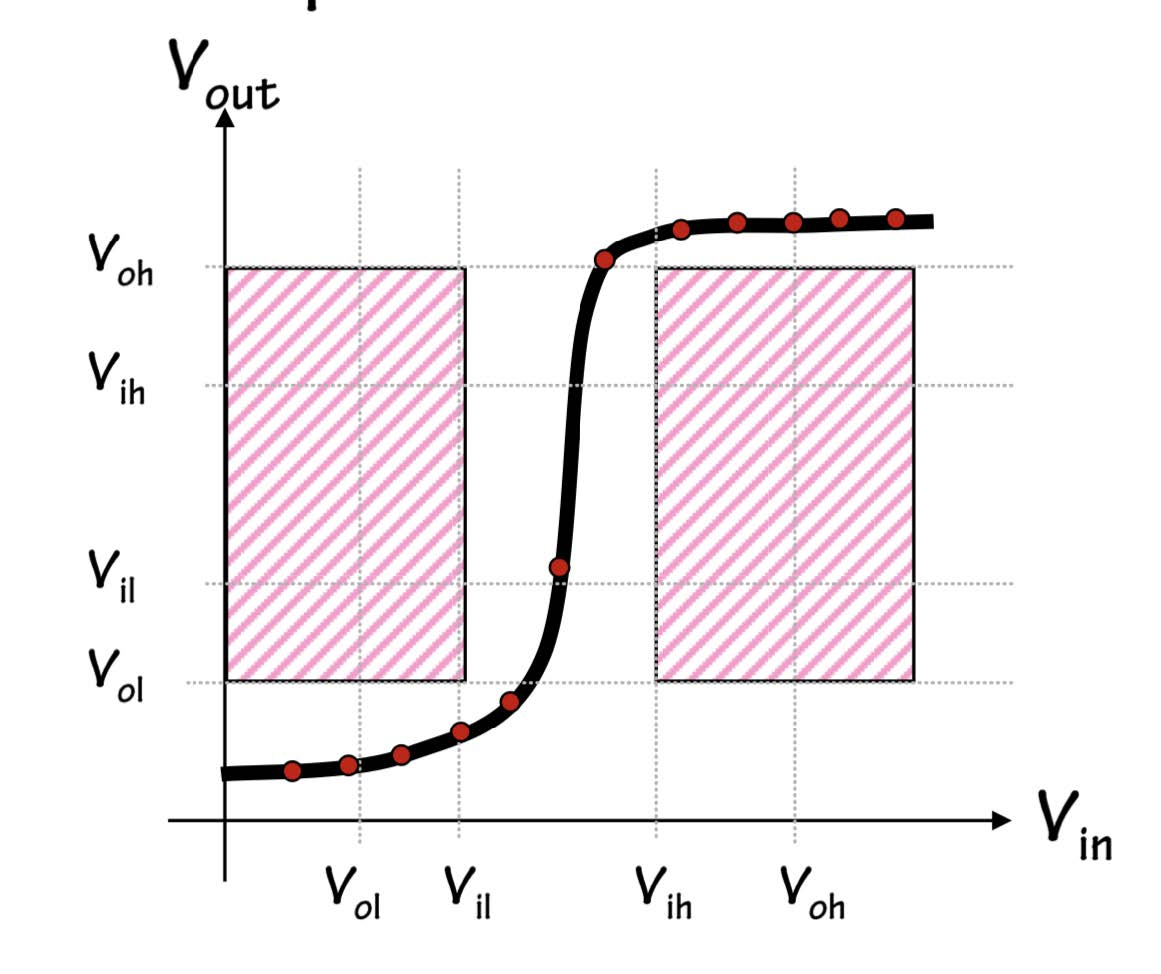
\includegraphics[width = 4.0cm]{VTC} \\
\begin{enumerate}
 \item Gain $>$ 1 (Because of static discipline)
 \item Non-Linear Gain
\end{enumerate}

\subsection{Noise Margin}
$V_{ol}$ or $V_{oh}$ is the voltage that your system outputs \\
$V_{ih}$ or $V_{ih}$ is the voltage that your system receive as input from another system.

\section{The MOSFET}
\begin{enumerate}
 \item The side with the higher potential is drain, the one with the lower potential
is source.
\item The p-type : majority care holes (impurities), bulk is connected to VDD
\item The n-type : majority are electrons, bulk is connected to GND
\item P0N1 (ON)
\end{enumerate}

\section{Timings}
\begin{enumerate}
 \item The Propagation Delay $t_{pd}$ - the time delay from valid input to valid output. The effective tpd of an entire
circuit is the maximum cumulative propagation delay over all paths from inputs to outputs.
\item The Contamination Delay $t_{cd}$ - the time delay from invalid input to invalid output. The effective tcd of an
entire circuit is the minimum cumulative contamination delay over all paths from
inputs to outputs.
\end{enumerate}
 
 \section{Logic Synthesis}
Universal:can implement any boolean function. 
 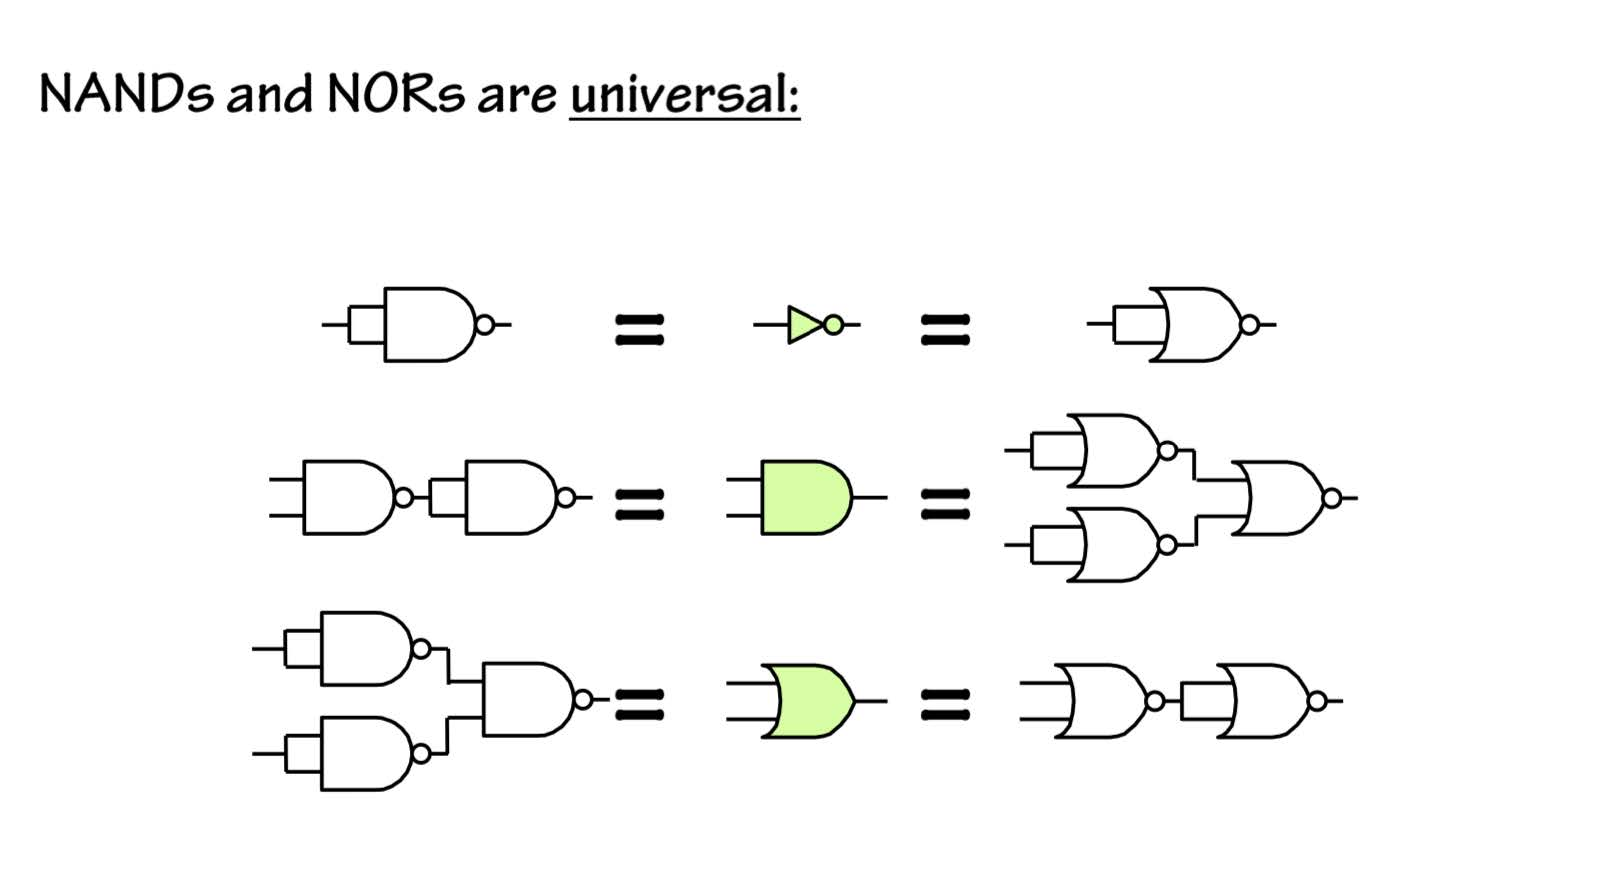
\includegraphics[width = 4.5cm]{NAND_NOR}
 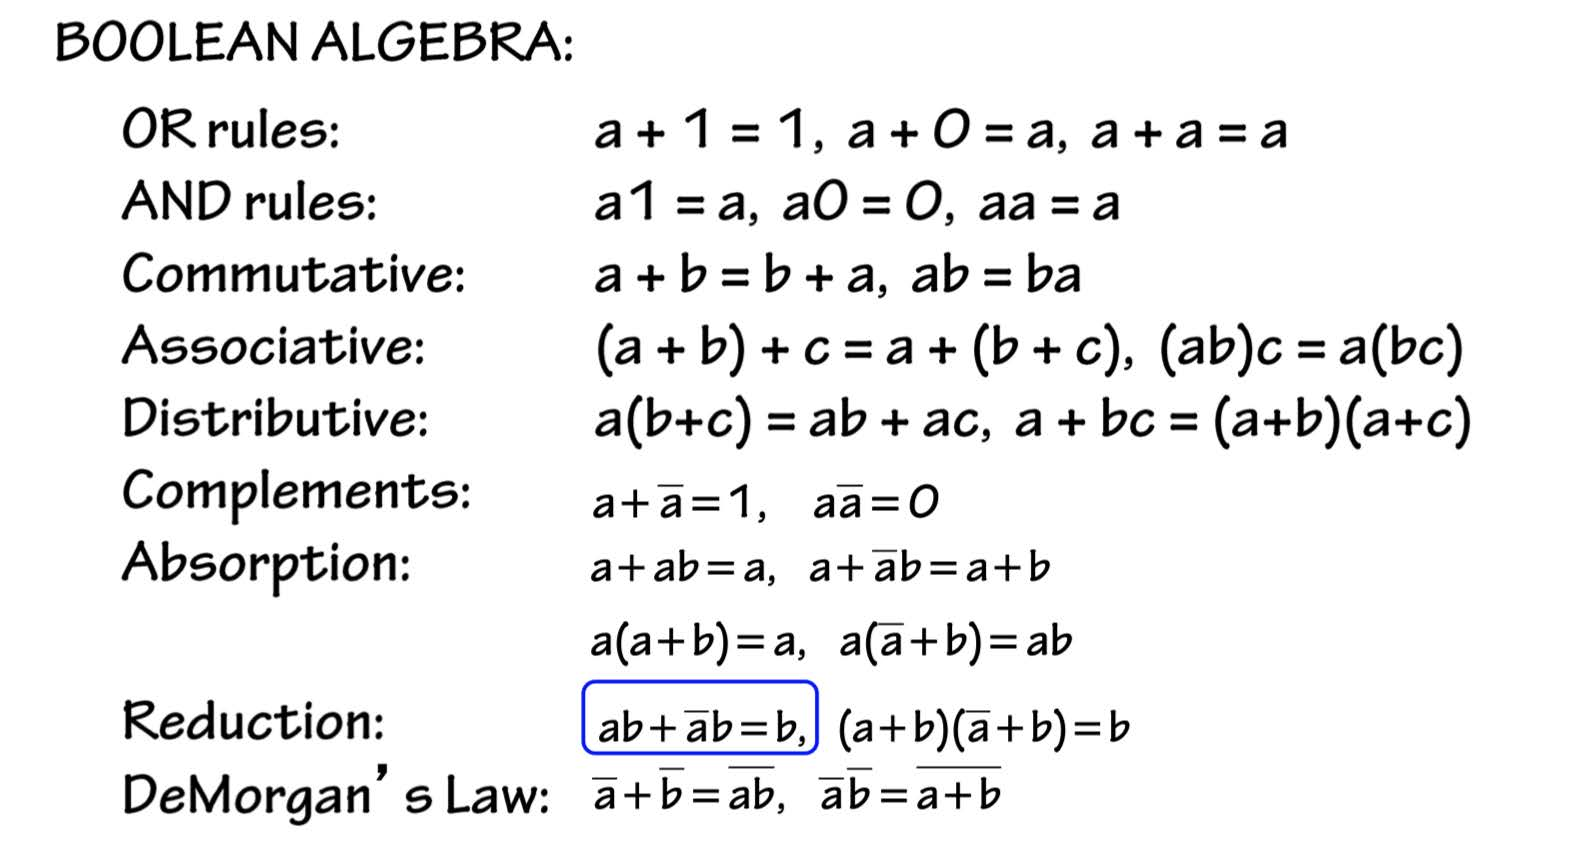
\includegraphics[width = 4.5cm]{boolean}
 \subsection{Karnaugh Map}
 \begin{enumerate}
\item ”1” cells, No diagonal grouping, Cells can overlap.
\item The top/bottom and left/right edges of map are continuous
\end{enumerate}
 
\section{Multiplexer (MUX)}
It is made up of logic gates (INV, AND, and OR, or
NANDs).\\
  \begin{itemize}
 \item Muxes are universal,
\item $2^{k}$ data inputs, k bits select inputs, and only can have 1
output
\item Three components: the inputs, the selector
signal(s), and the output. 
\end{itemize}
 \section{Decoder}
\begin{enumerate}
 \item A Decoder is the opposite of Mux
\item It has k select inputs, and $2^{k}$ possible data outputs
\item The selected output i is HIGH (1), and the rest of the $2^{k} - 1$ data output is LOW
(0).
\end{enumerate}
\subsection{Read-Only-Memories (ROM)}
\begin{enumerate}
\item For an N-input boolean function, the size of ROM is roughly $2^{N}$ X  number of outputs.
FA: $2^{3}*2$ = 16
\end{enumerate}

\section{The Dynamic Discipline}
The input to a synchronous sequential circuit must be stable
during the aperture (setup and hold) time around the clock
edge.
The dynamic discipline states that
\begin{enumerate}
\item $T_{setup} = 2t_{pd}$
\item $T_{hold} = t_{pd}$
\end{enumerate}
\begin{enumerate}
\item $T_{setup}$ = the minimum amount of time that the voltage on wire D needs to be stable before the clock edge changes from 0 to 1.
\item $T_{hold}$ = the minimum amount of time that the voltage on wire D needs to be stable after the clock edge changes from 0 to 1.
\item $t_{pd}$ is the propagation delay of the D-latch
\end{enumerate}
\section{Flip-Flop}
Created by putting 2 D-latches in series \\

\begin{enumerate}
\item There is an inverter on the G input on the master flip flop
\item When CLK signal is 0, the G wire of master latch receive a 1 while slave flip flop receive a 0 \\
Master latch : Write mode \\
Slave latch : Read mode
\item Vice-versa when CLk signal is 1
\item 1 D-Latch is on write mode why 1 D-latch is on memory mode at anytime.
\end{enumerate}
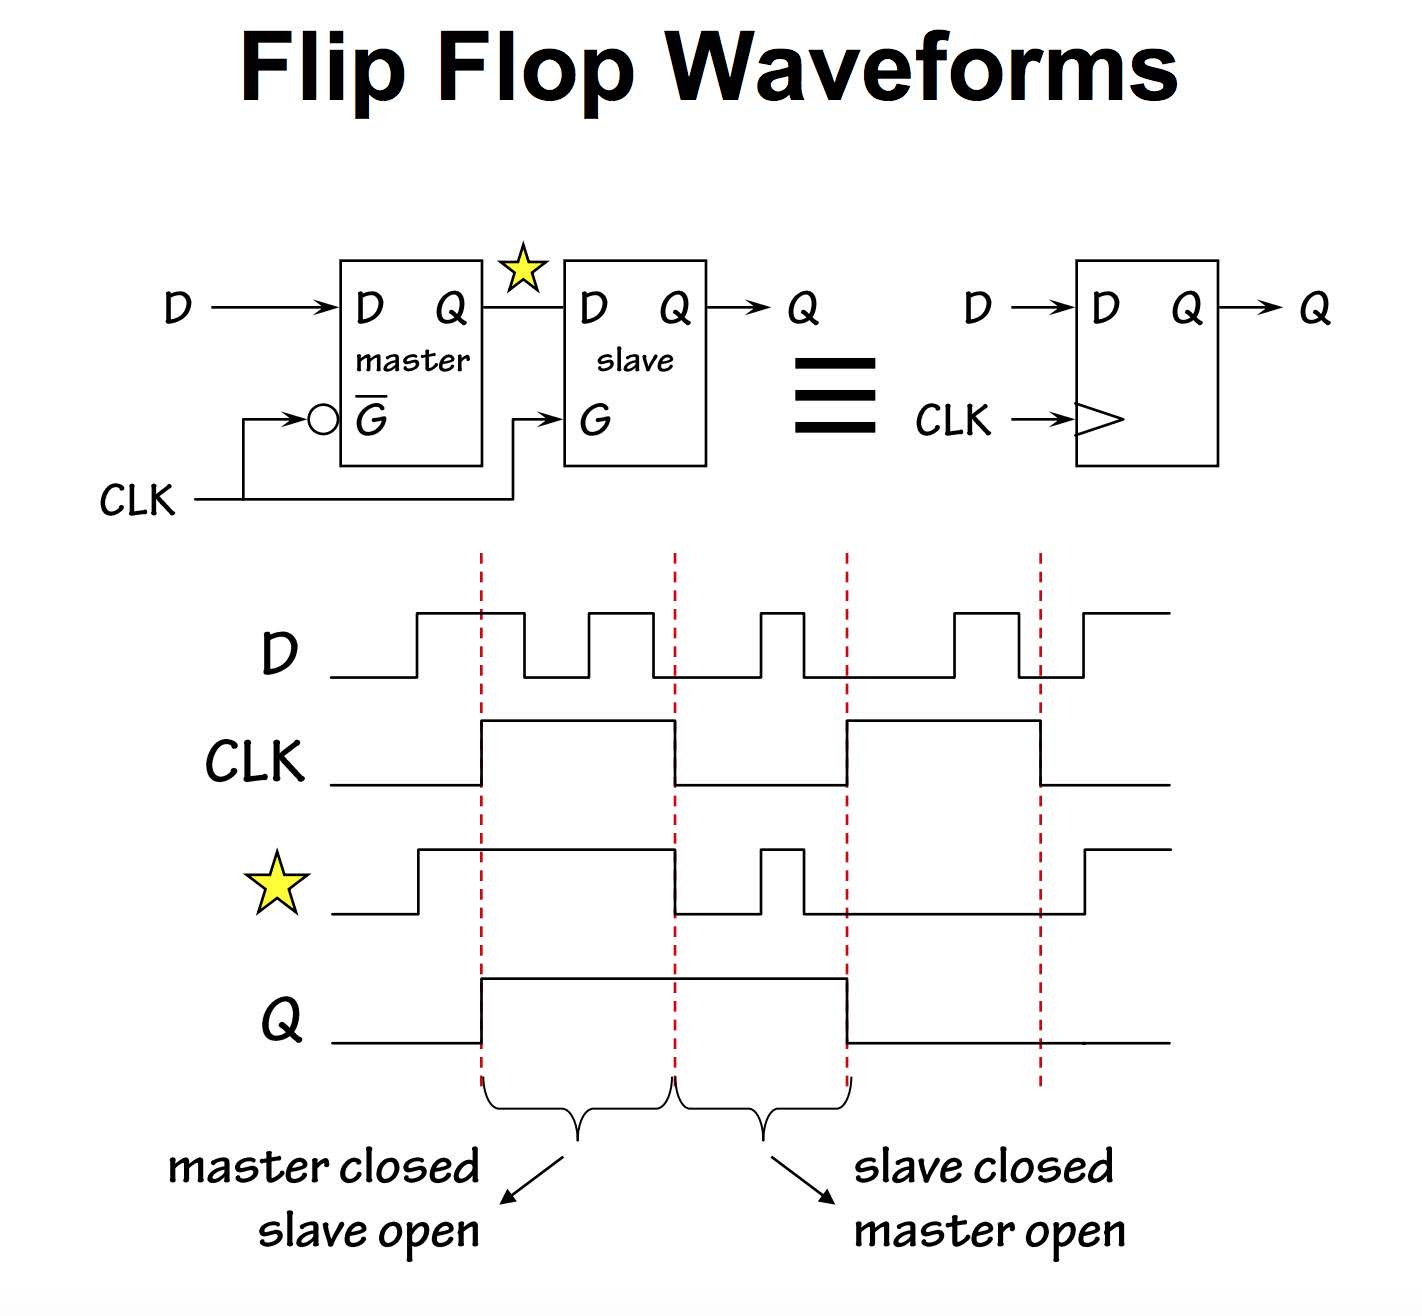
\includegraphics[width = 4.5cm]{Flip_flop_waveform}
Note that output wire Q only changes when CLK rises from 0 to 1
\subsubsection{Timing Constraint}
\begin{enumerate}
\item $t_{CD}$ of a D-latch is the time taken for invalid CLK input to produce an invalid output on wire G
\item $T_{PD}$ of a D-latch is the time taken for valid CLK input to produce a valid output on wire G
\end{enumerate}

Sequential Logic Timing Constraint
$t_{1} = t_{CD,R1} + t_{CD,1} > t_{HOLD,R2}$
$t_{2} = t_{PD,R1} + t_{PD,1} < t_{CLK} - t_{SETUP,R2}$


\section{Metastable State}
Properties
\begin{enumerate}
\item It corresponds to an invalid logic level
\item Unstable equilibrium which will settle to valid 0 or 1 eventually
\item Settling can be arbitraily long
\item All bistable system exhibits at least 1 metastable state
\item Cannot be avoided but can be minimize
\end{enumerate}

\subsubsection{Clock Skew}
$t_{1} = t_{CD,R1} + t_{CD,R1} > t_{HOLD,R2} + t_{skew}$ \\
$t_{2} = t_{PD,R1} + t_{PD,CL1} < t_{CLK} - t_{SETUP,R2} + t_{skew}$ \\


\section{Programmable Machines}

\subsection{Finate State Machine: Enumeration}
FSM with \textit{i} inputs, \textit{o} outputs, \textit{s} states 
\begin{enumerate}
\item Truth table has $2^{i + s}$ rows with (o + s) columns each
\item $2^{(o + s) 2^{i + s}}$ max state
\item Limitation : cannot solve problems with arbitrarily many states
\end{enumerate}

\subsection{MOORE MEALY}
Moore: output drawn on states and depends only on state. 
Arcs leaving must be mutually exclusive and colletively exhaustive

\subsection{Turing Machines}
Turing Machine Specification
\begin{enumerate}
\item Doubly-infinite tape
\item Discrete symbol positions
\item Finite alphabet
\item Control FSM \\
Inputs - Current Symbol \\
Outputs - Write 0/1 , move Left/Right 
\item Start State , Halt State
\end{enumerate}
Properties
\begin{enumerate}
\item Can be used to compute integer functions of form $y = T_{k}[x]$ 
\item Where k: FSM index, x: input tape configuration, y: output tape configuration. \\
*Not all integer functions can be computed with Turing Machines
\item Computable functions : f(x) computable $\Leftrightarrow \exists k : \forall x: f(x) = T_{k}[x] = f_{k}(x)$
\item Church-Turing Hypothesis states that any computable function is computable by a TM
\end{enumerate}

\subsection{Universal Functions and Universality}
Universal function: $U(k,j) = T_{k}(j)$ \\
U is comptable by a Turing Machine \\
$\rightarrow$ k encodes a 'program' \\
$\rightarrow$ j encodes the input data to be used \\
$\rightarrow T_{u}$ interprets program

\section{Von Neumann Model}
4 components
\begin{enumerate}
\item CPU - contains several registers as well as logic
\item Memory = storage of N words with W bits, where W is a fixed architerctural paramter, and N can be expanded to meet needs
\item Input/Output 
\item Connection Bus
\end{enumerate}

\section{Week 5}
\section{Machine Language and Compilers}
\subsection{Compiler}
\begin{enumerate}
\item Complier translate high-level language into low-level assembler machine language
\item Done before execution and slows program development
\item Decisions made during compile time,before execution
\end{enumerate}
\subsection{Interpreter}
\begin{enumerate}
\item Computes exact instructinos
\item Done after execution and slows down program execution
\item Decisions made during run time, after execution
\end{enumerate}

\section{Week 8}
\subsection{CPU Design Tradeoffs}
\begin{enumerate}
\item Maximum Performance
\item Minimum Cost
\item Best Performance - MIPS = $\frac{Clock Frequency (MHz)}{clocks per instruction}$
\end{enumerate}
Instruction classes - OP,OPC,MEM,Transfer of Control 

\subsection{Multi-Port Register Files}
\begin{enumerate}
\item 2 combinational Read ports
\item 1 clocked Write port - Write Address,Write Data,Write Enable
\end{enumerate}
\subsection{Exception}
Bad Opcode \\ Reg[XP] $\leftarrow$ PC + 4 , PC $\leftarrow$  illOp \\
Other \\ Reg[XP] $\leftarrow$ PC + 4 , PC $\leftarrow$  Xadr \\

\subsection{Extending Beta}
\subsubsection{LDX(R0,R1,R2)}
ADD(R1,R0,R0) ,
LD(R0,0,R2) \\
Reg[Rc] $\leftarrow$ Mem[ Reg[Ra] + Reg[Rb]
\subsubsection{STX(R0,R1,R2)}
ADD(R1,R0,R0) ,
ST(R2,0,R0) \\
Mem[ Reg[Ra] + Reg[Rb] ] $\leftarrow$ Reg[Rc] \\
Must amend data path and register file! 
Register file needs another RA/RD port. RA2SEL mux can be removed.

\section{Week 9}
\section{Memory Hierarchy}
From fastest and most expensive: Cache,SRAM,DRAM, Hard desk \\
Both SRAM and DRAM are volatile storage
\subsection{SRAM}
Static RAM 
\begin{enumerate}
\item 6 transitors and amp sense in each cell with 2 bit line
\item Value stays the same if word line is 0
\item Store a bit
\end{enumerate}
\subsection{DRAM}
\begin{enumerate}
\item 1 transitors ,a capacitor and store a bit
\item A lot cheaper but significantly slower.
\end{enumerate}
\subsection{Disk}
SSD/HDD \\
Non volatile storage (Can store information even after power source is cut)

\section{The Cache Idea}
\begin{enumerate}
\item Look for requested info in cache
\item If found, it's a hit. Else, go to physical memory and subsequently disk.
\end{enumerate}
\subsection{Locality of references}
Reference to memory location X at time t implies that reference to X + change(X) at
t +change(t) becomes more probable as change(X);change(t) approaches zero.

\section{Type of Cache}
\subsection{Fully Associative Cache(FA)}
Pros: Parallel Lookup and Flexible,address can be stored on any cache line \\
Cons: Needs many Bool operator(1 for each cache line). Also need a replacement strategy. \\ 
\begin{enumerate}
\item TAG contains the all bits of address A
\item DATA contains all bits of content at A: Mem[A]
\item Expensive, made up of SRAMS and other hardwares (comparator circuit
at each row)
\item PARALLEL lookup, hence making it fast
\item Flexible because memory address + content can be stored on any TAG-DATA
row.
\item Need replacement strategy
\end{enumerate}

\subsection{Direct mapping Cache(DM)}
Pros: Cheaper as only 1 Bool operator , No need replacement strategy\\
Cons: Contention - \\
\begin{enumerate}
\item TAG contains T-upper bits of address A
\item DATA contains all bits of content at A: Mem[A]. Lower K-bits of A decides
row of DM Cache. Mapped to exactly one of the rows of DM cache.
\item Also made of SRAMS but cheaper than FA cache(only one comparator circuit per DM cache)
\item No parallelism, but fast mapping between address and cache line
index 
\item Suffers contention, two different addresses can be mapped to the same location when the K-lower bits are the same. K-lower bits selected due to locality of reference, but does not completely eliminate contention.
\end{enumerate}



\subsection{Cache Design Issues}
\begin{itemize}
\item Associativity : how many different address can be stored in the cache
\item Replacement strategy
\item Block size
\item Write strategy
\end{itemize}

\subsection{N-way set associative cache}
\begin{enumerate}
\item if N = 1, it is a DM cache.
\item if k = 1, it is a FA cache
\item Same Column $\implies$ same cache line
\item k lower bits determines the set in which it will be in. 
\end{enumerate}


\subsection{Replacement Strategy}
\begin{enumerate}
\item Least Recently Used: overhead is O(N$\log_{2}{N}$)
\item FIFO: O($log_{2}{N}$) bits/set
\item Random - uses psedu random generator to get reproducible behavior
\end{enumerate}

\subsection{Block Size}
Blocks of $2^{B}$ words per row,

\subsection{Special Bits}
\subsubsection{Valid Bit}
The valid bit indicates that the particular cache row (also called cache line, but it
is a different graphical representation from ’cache line’ in the N-way set associative
cache) contains data from memory and not empty or redundant value. We only
check cache lines with valid bit = 1.
\subsubsection{Dirty Bit}
The dirty bit is set to 1 iff the CPU writes to cache and it hasn’t been stored to the
memory (memory is outdated).
\subsubsection{LRU}
The LRU bit is present in each cache line (for FA), and each cache set-cacheline cell
(for NW), regardless of the block size because R/W with block size more than 1
is always done in parallel.

\section{Cache Writes}
\subsection{Write-through}
CPU writes are done in the cache first by setting TAG = Addr, and Data = new
Mem[Addr] in an available cache line, but also written to the main memory immediately.
This stalls the CPU until write to memory is complete, but memory always
holds the ”truth”
\subsection{Write-behind}
Write to the main memory is buffered or pipelined. CPU keeps executing next instructions while writes are
completed (in order) in the background. 
\subsection{Write-back}
Not immediately written to the main memory. Memory
contents can be ”stale”. Typically CPU will write to the main memory only if the
data in cache line needs to be replaced and that this data has been changed or is
new. This requires the dirty bit in the cache.

\section{MMU Details}
\begin{enumerate}
\item $2^{v + p}$ bytes of VM
\item $2^{m + p}$ bytes of actual memory
\item (m + 2) $2^{v}$ bits in MMU Pagetable
\item $2^{p}$ bytes per page
\end{enumerate}

\section{Page-Map Design}
Residence Bit - if R is 1, data is in RAM \\
Dirty Bit: if D is 1, data has to be written to Disk before removed from RAM

\section{TLB}
Cache to pagetable for mapping certain VPN to PPN. Locality of reference in address memory reference patterns. 

\section{Cache with VM}
Each cache line stores a single data (not pages) and the address of each data.


\end{multicols*}

\begin{multicols*}{5}
\setlength{\premulticols}{1pt}
\setlength{\postmulticols}{1pt}
\setlength{\multicolsep}{1pt}
\setlength{\columnsep}{2pt}

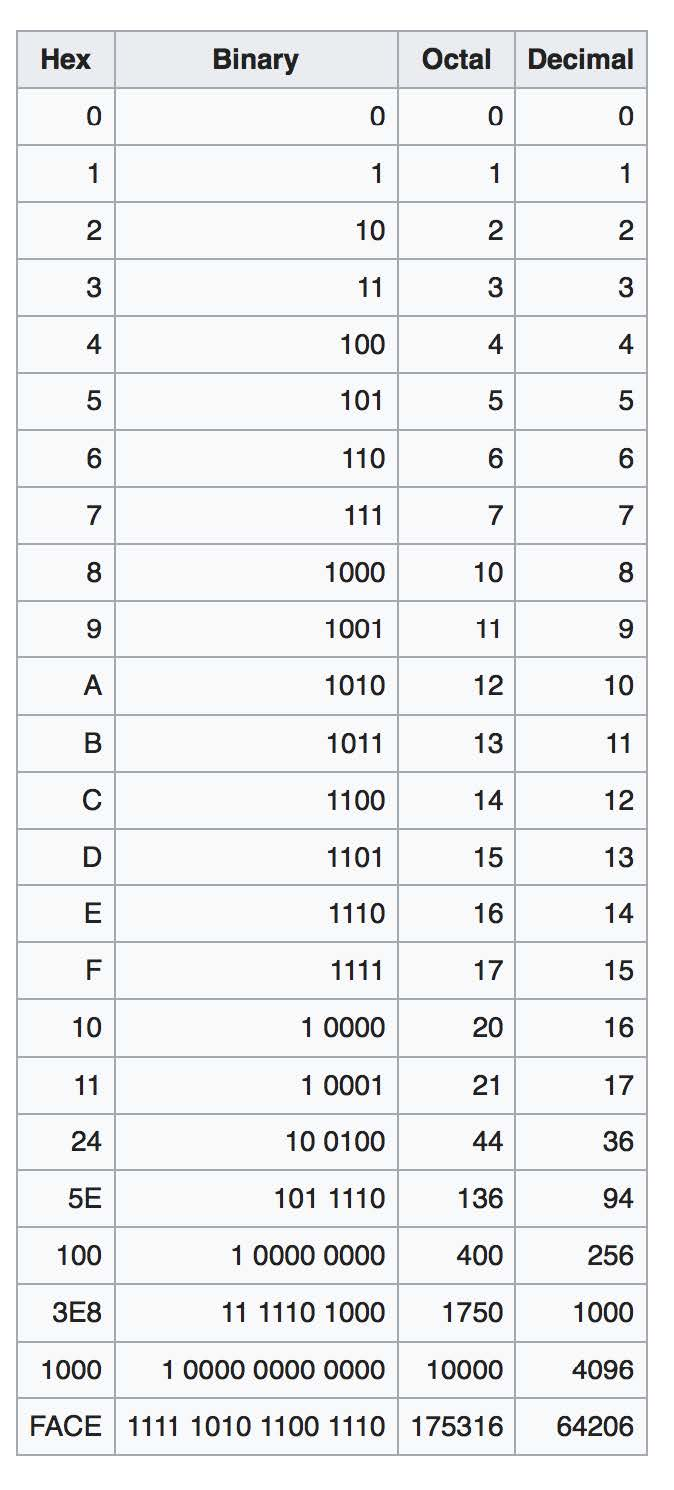
\includegraphics[width = 5cm]{Conversion_table}
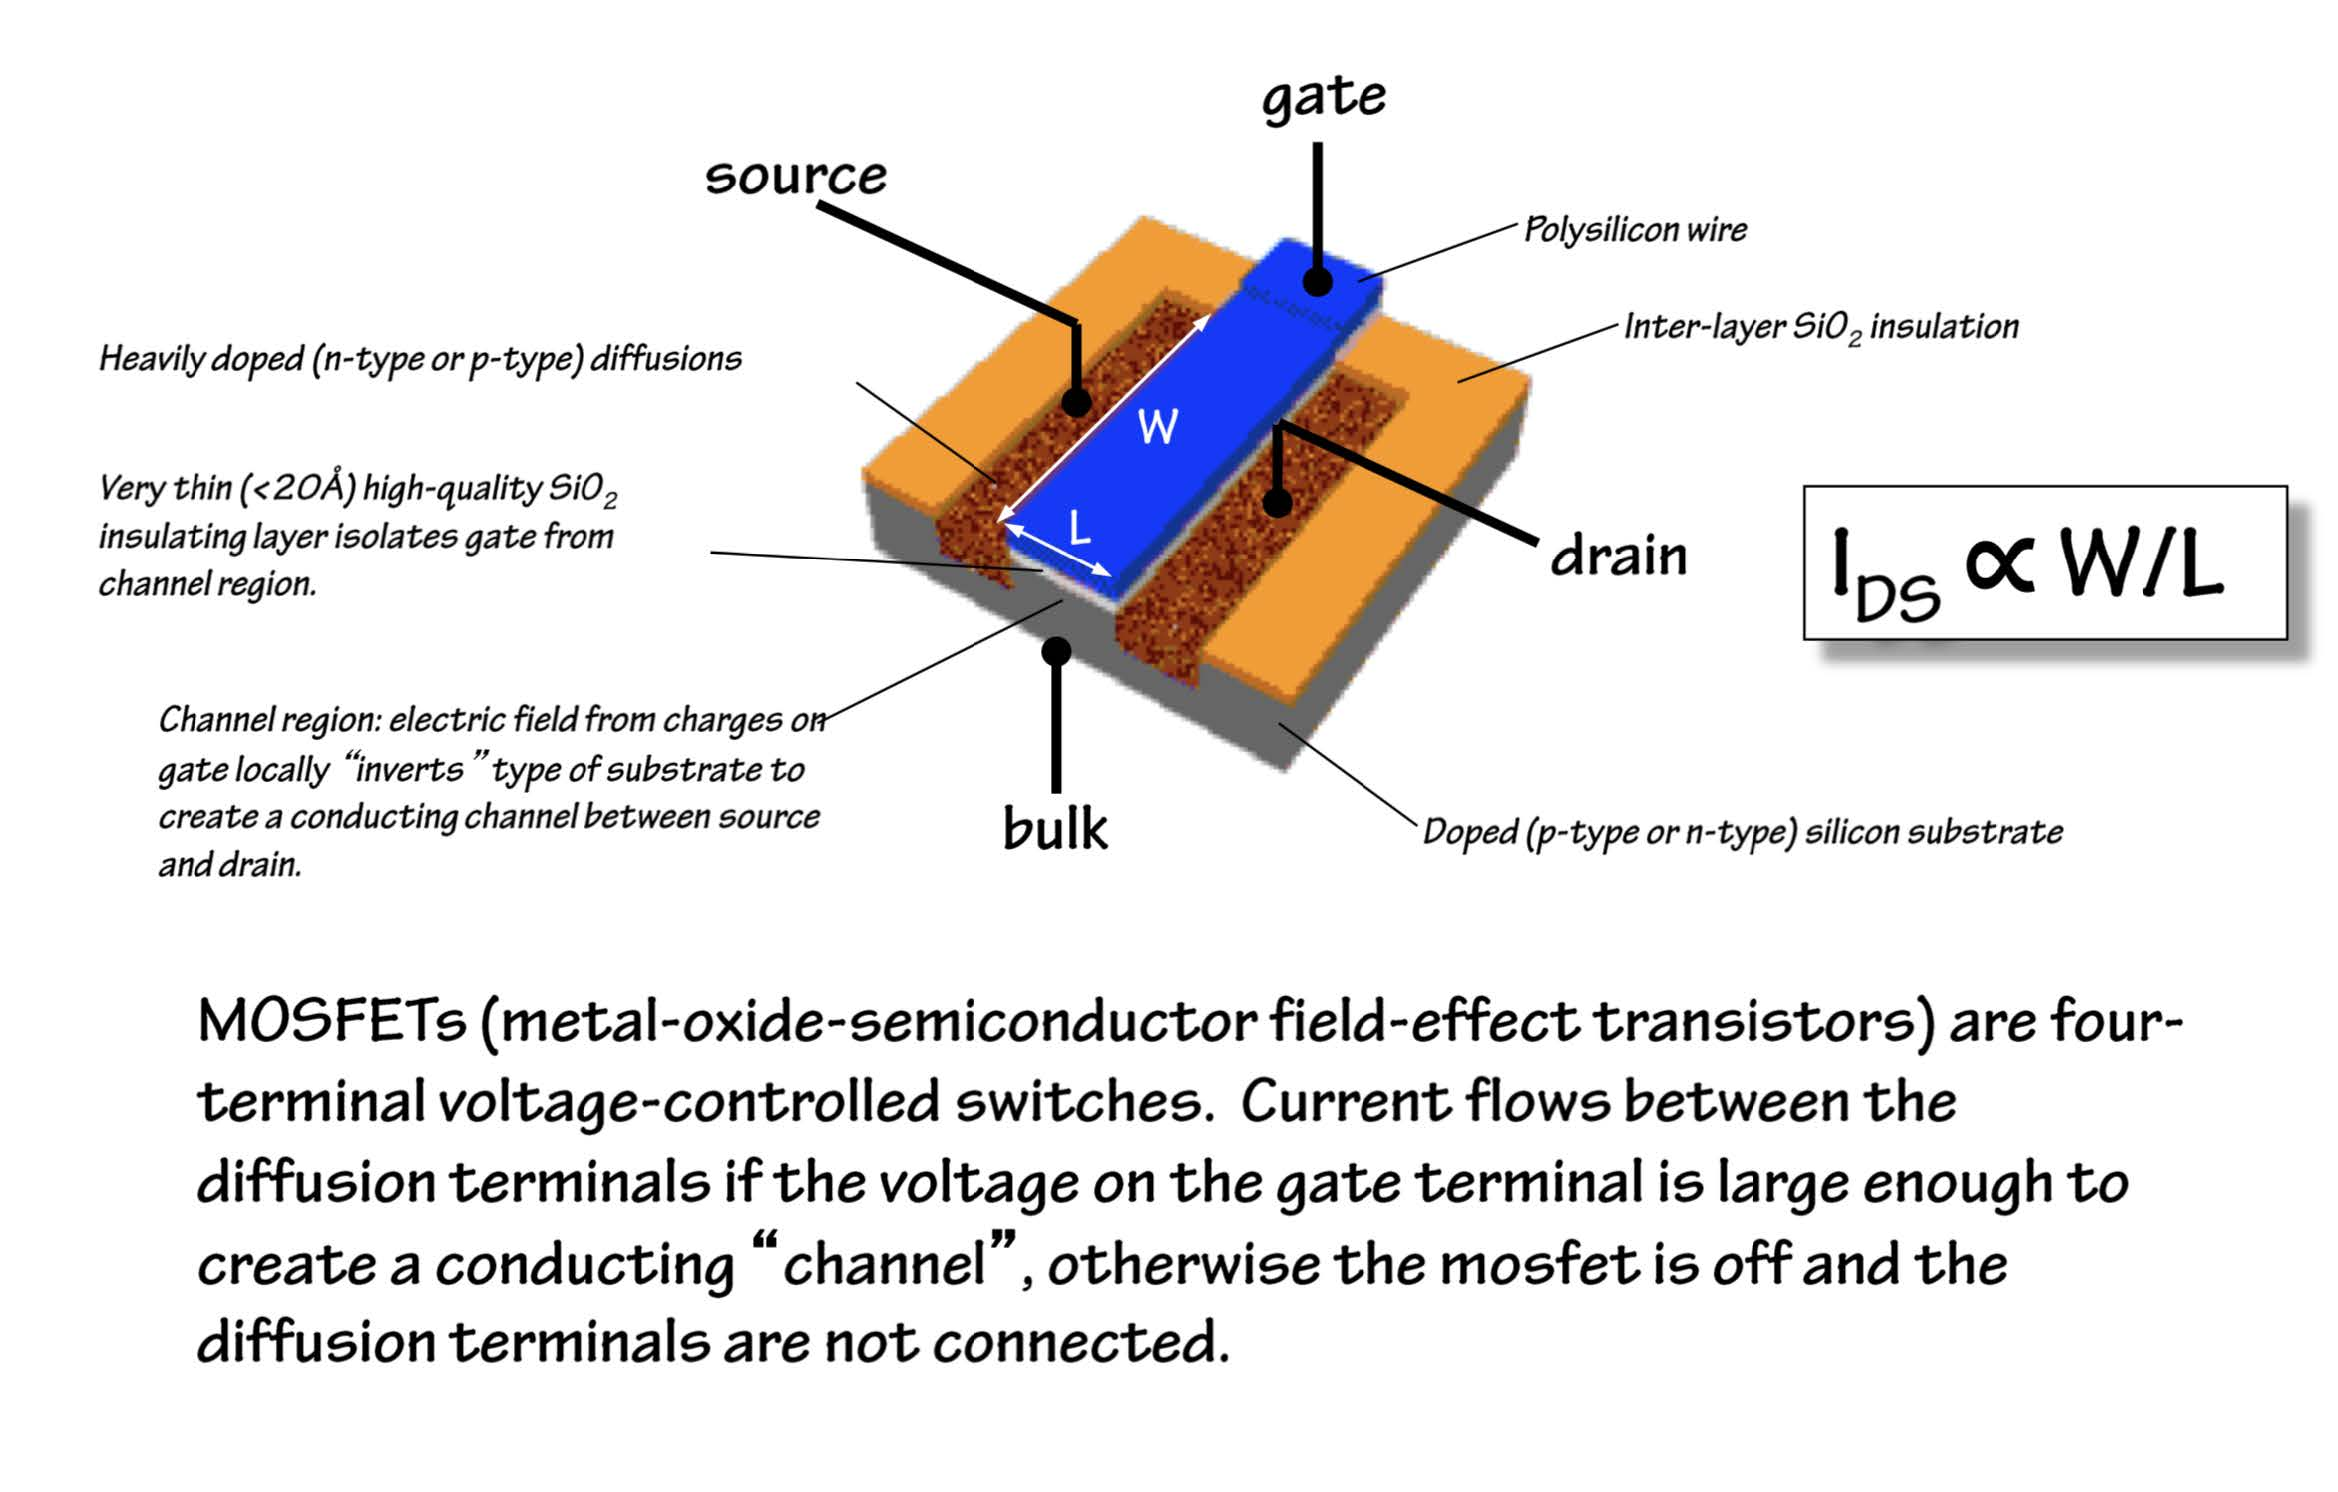
\includegraphics[width = 5.5cm]{Mosfet}
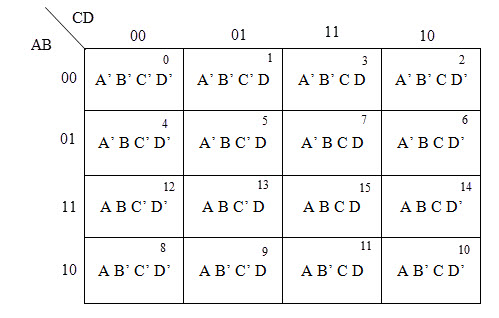
\includegraphics[width = 5.5cm]{K-map}
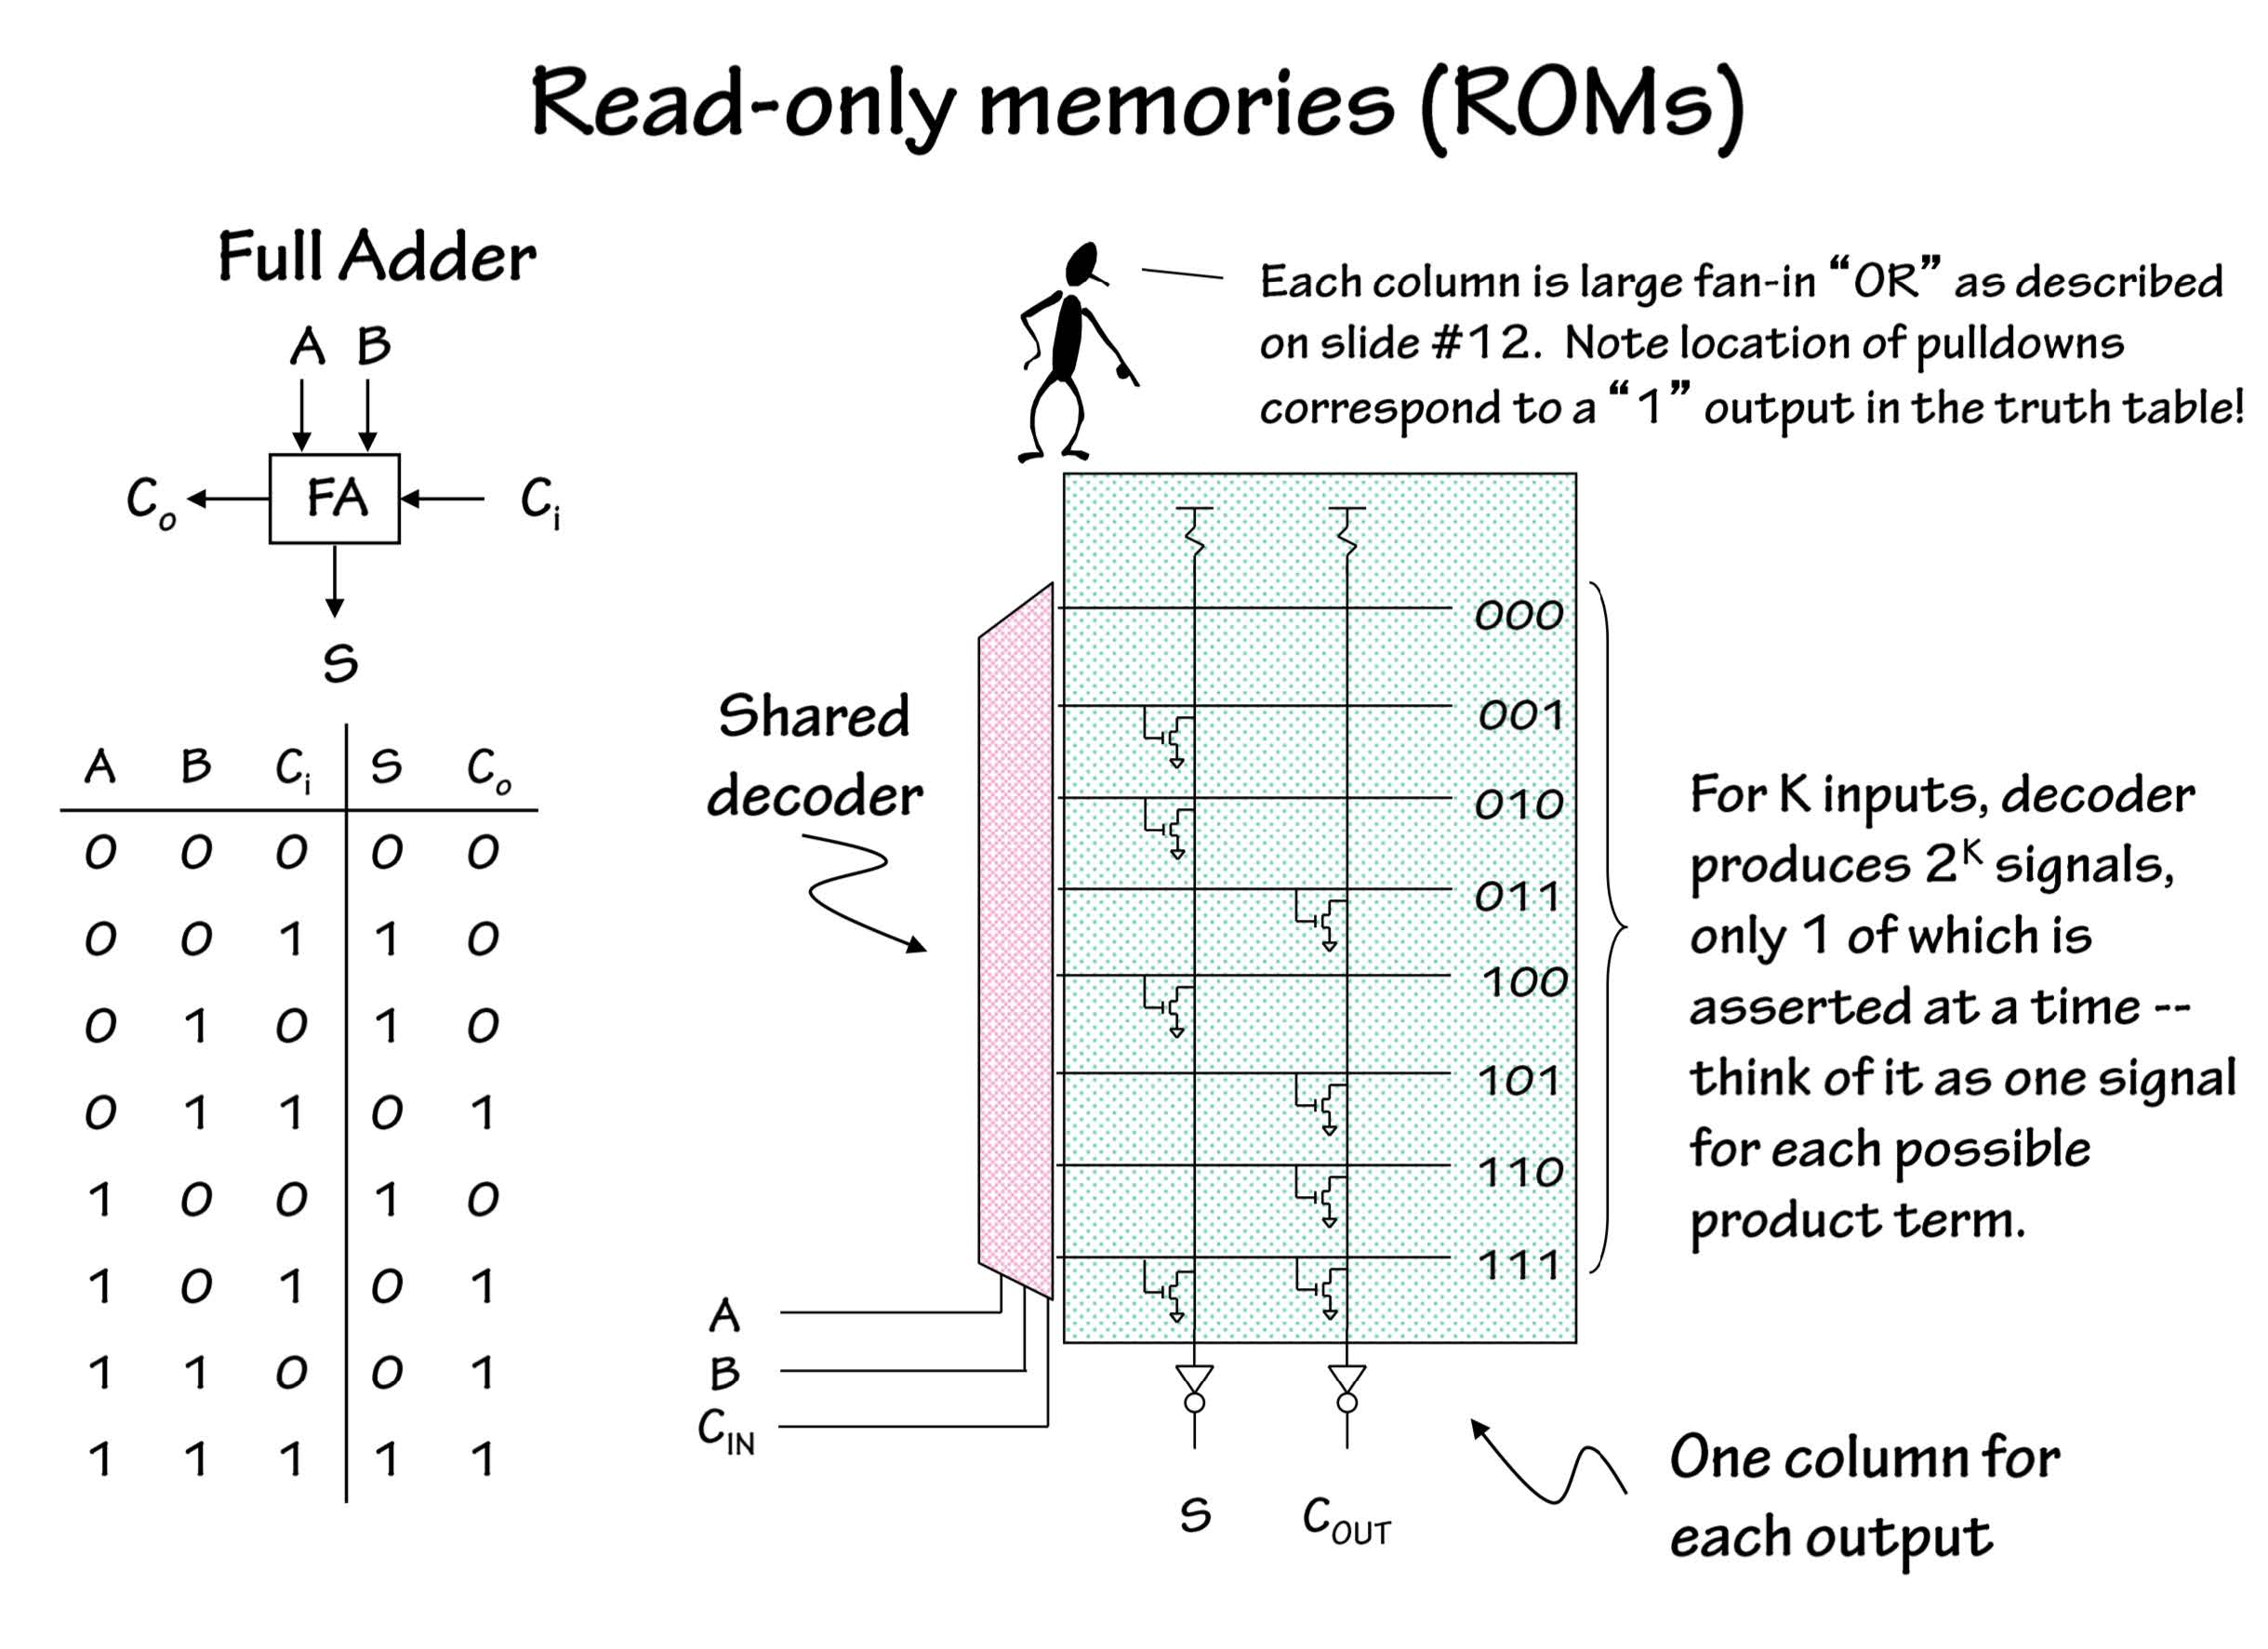
\includegraphics[width = 5.5cm]{ROM}
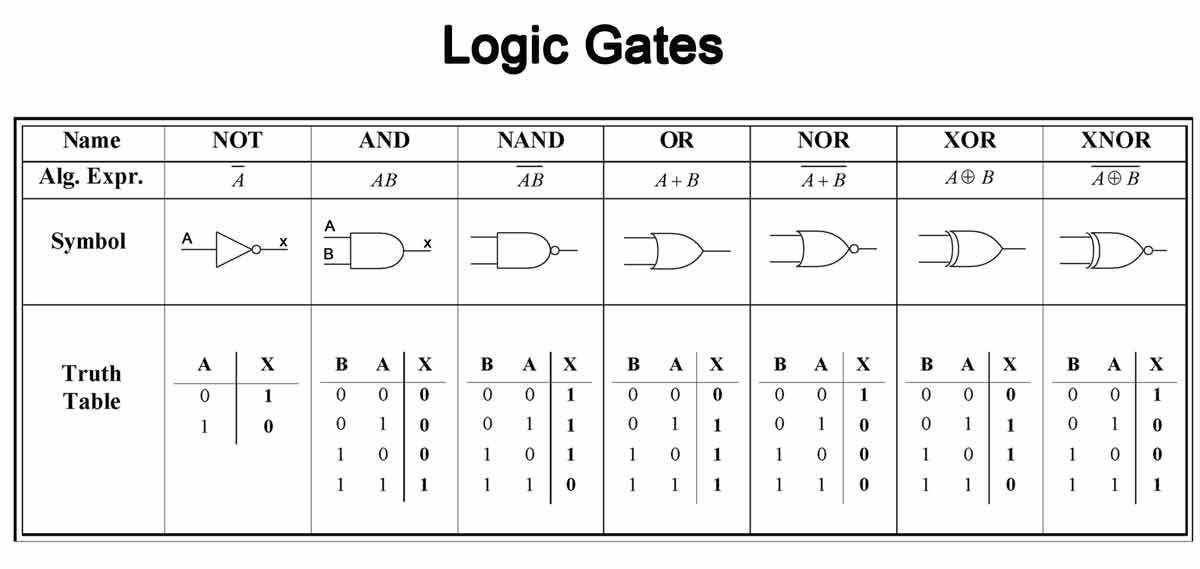
\includegraphics[width = 5.5cm]{Logic_gates}
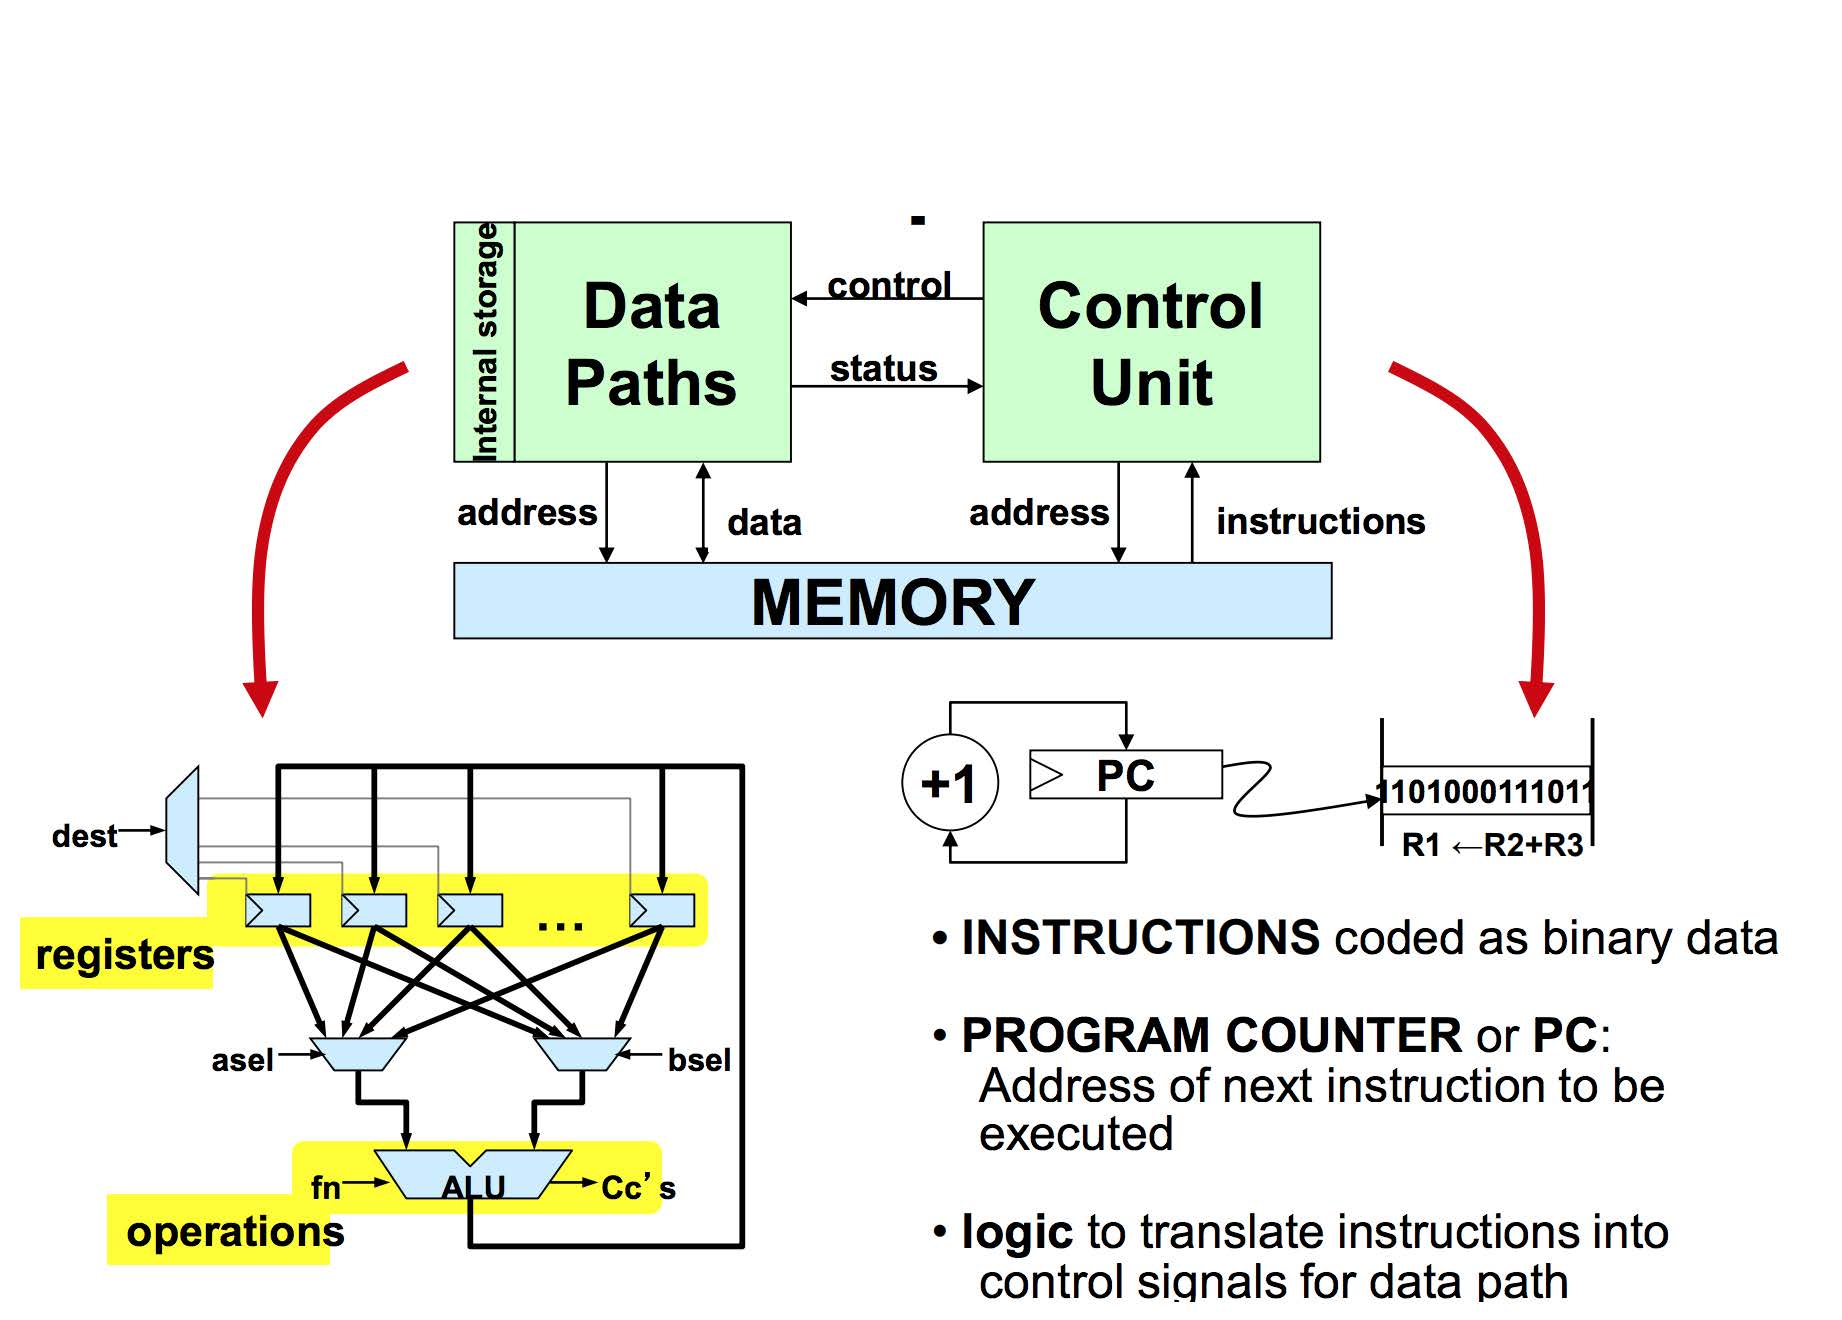
\includegraphics[width = 5.5cm]{CPU_anatomy}
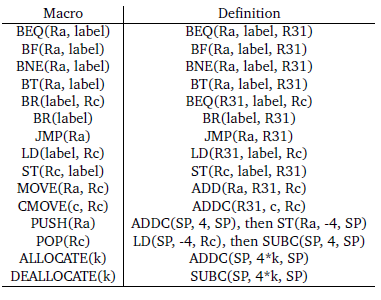
\includegraphics[width = 5.5cm]{Macro}
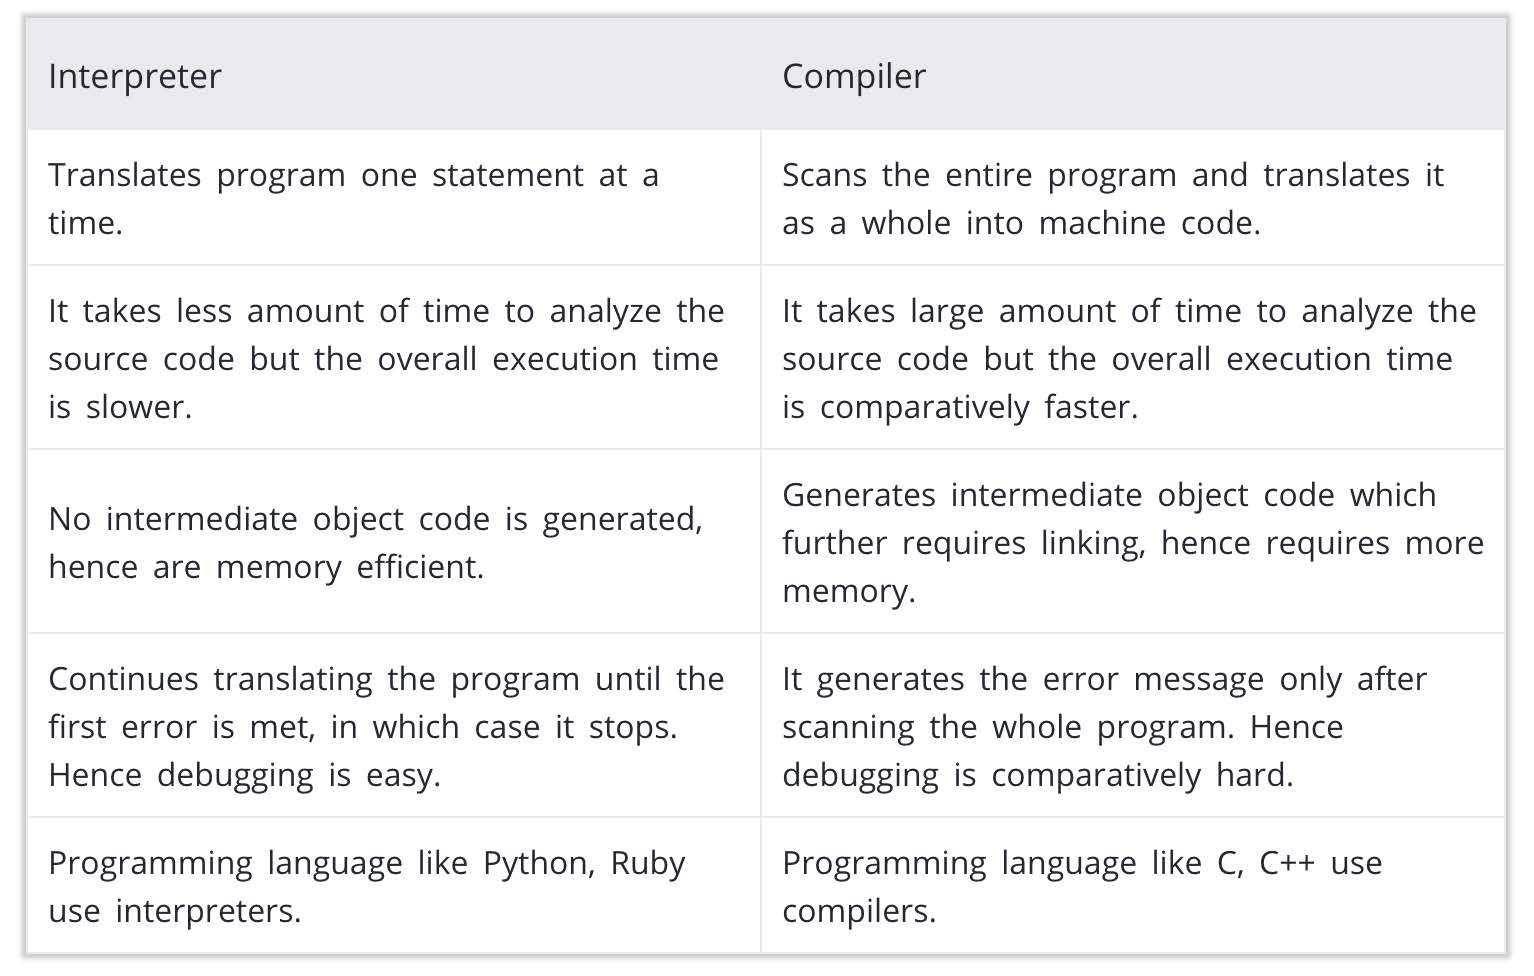
\includegraphics[width = 5.5cm]{Interpreter_Compiler}
\includegraphics[width = 5.5cm]{Cache_algo}
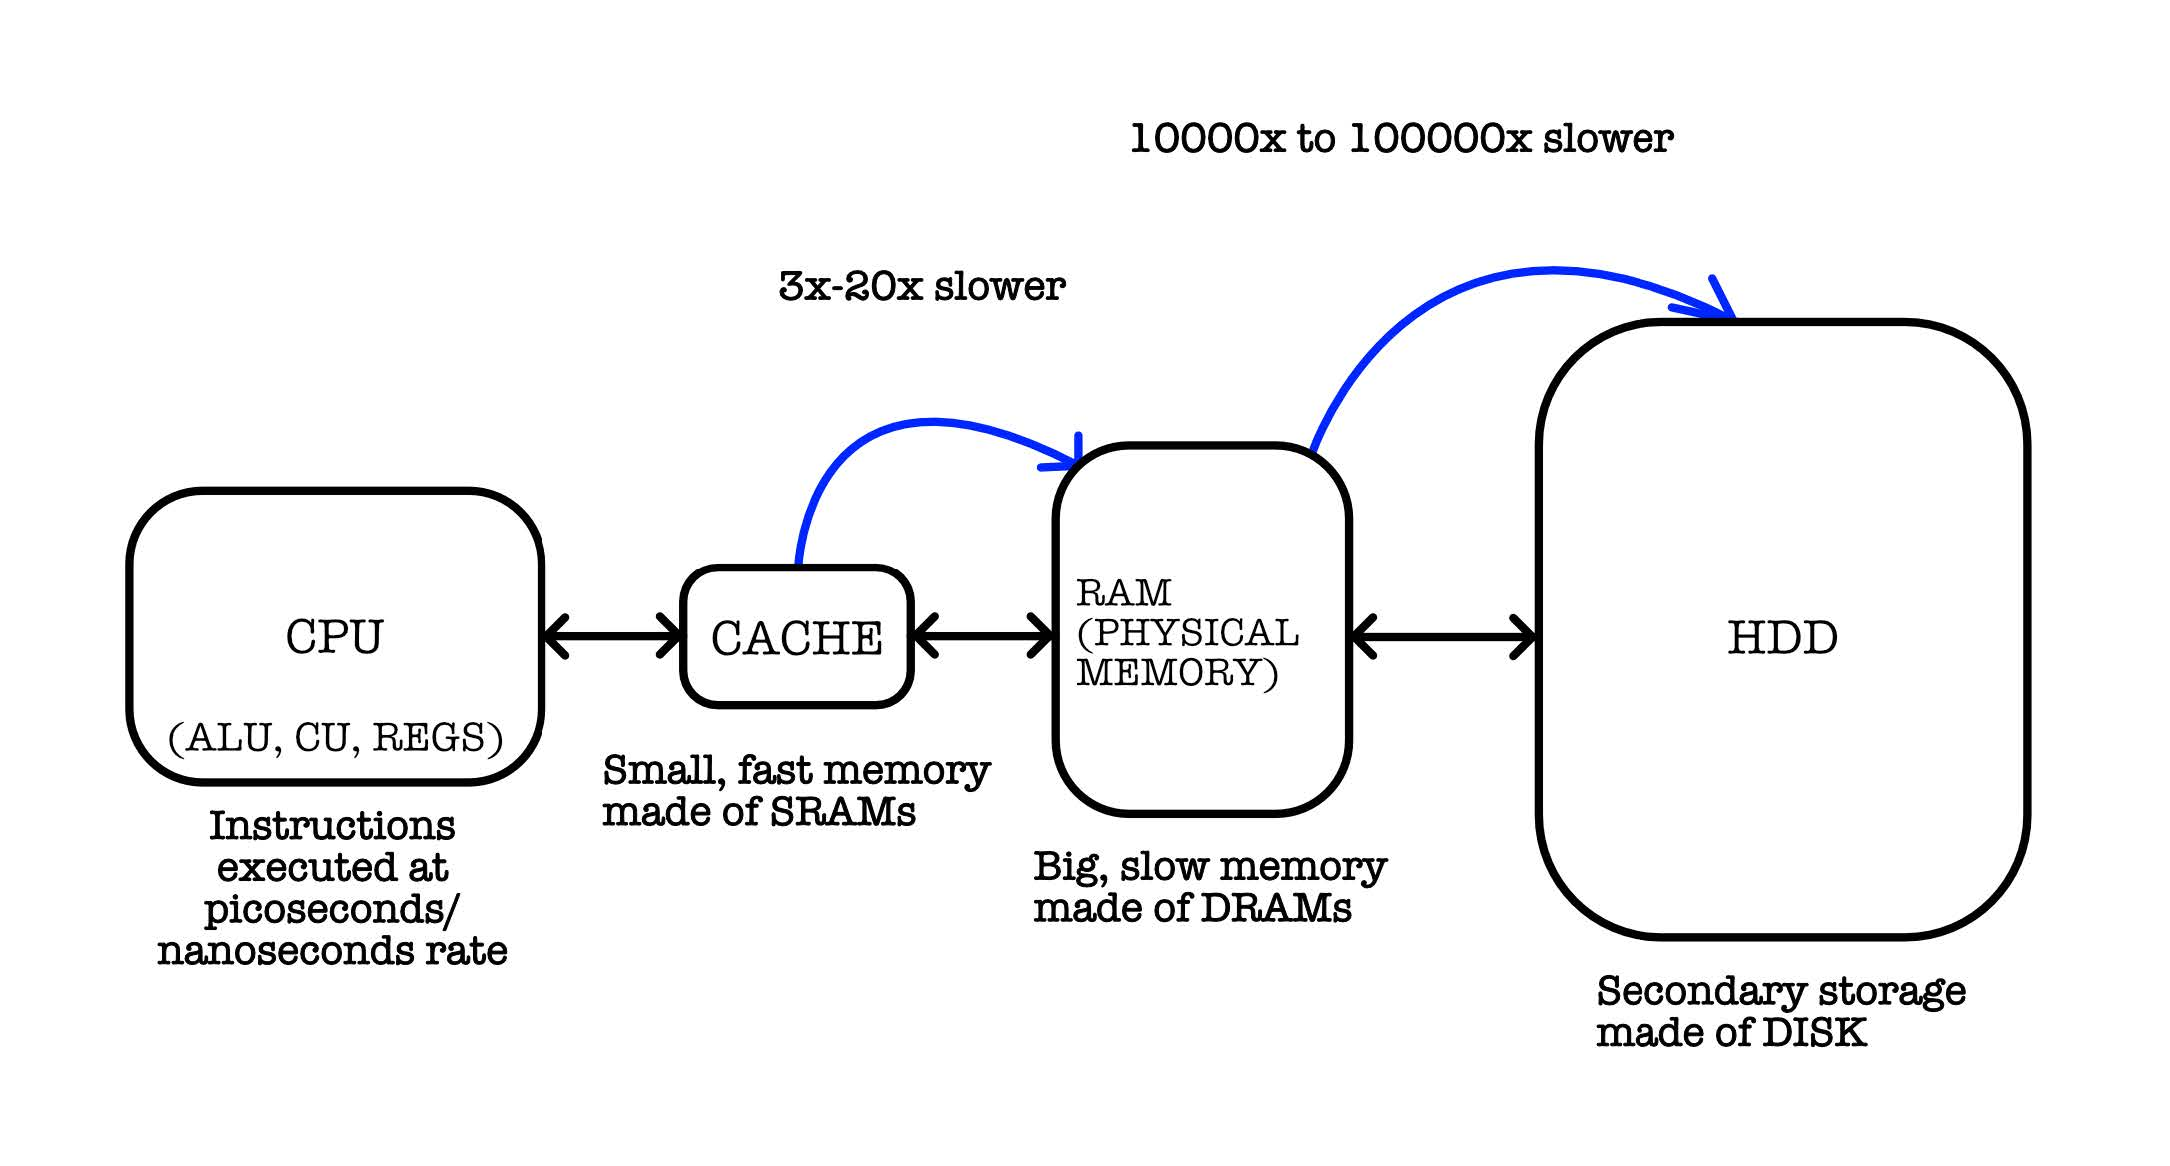
\includegraphics[width = 5.5cm]{MemoryHierarchy}
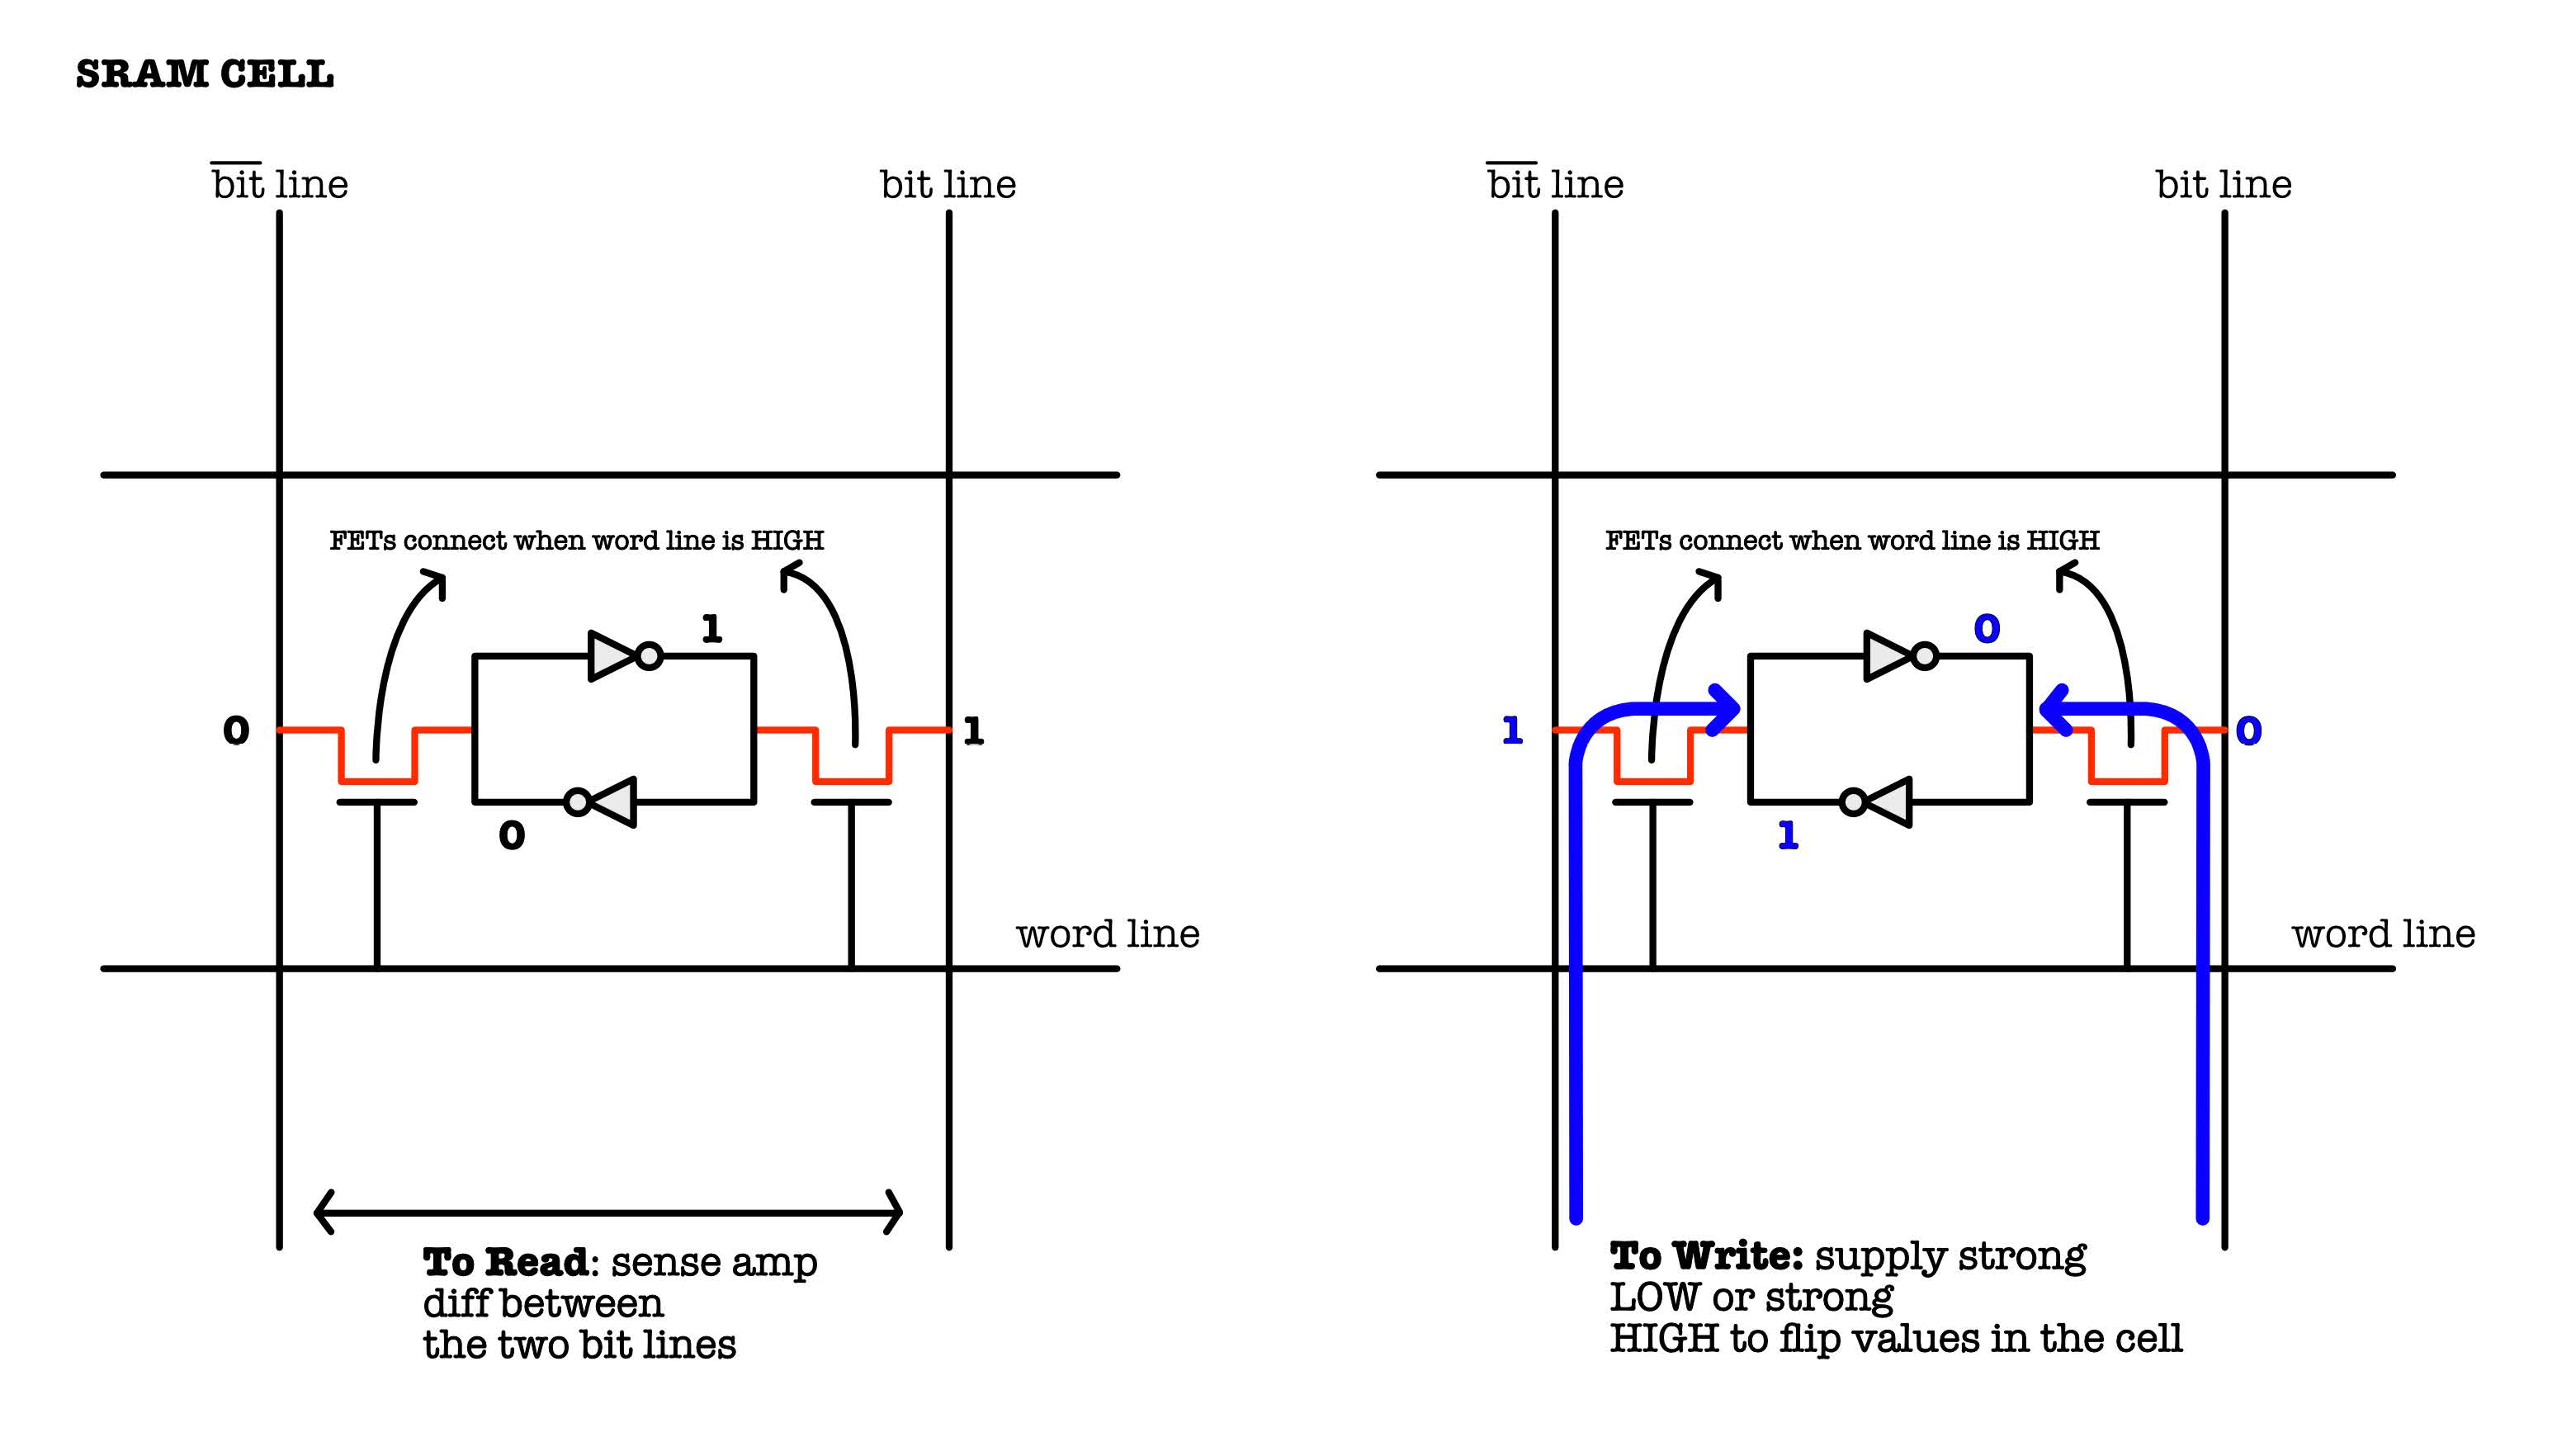
\includegraphics[width = 5.5cm]{SRAM_cell}
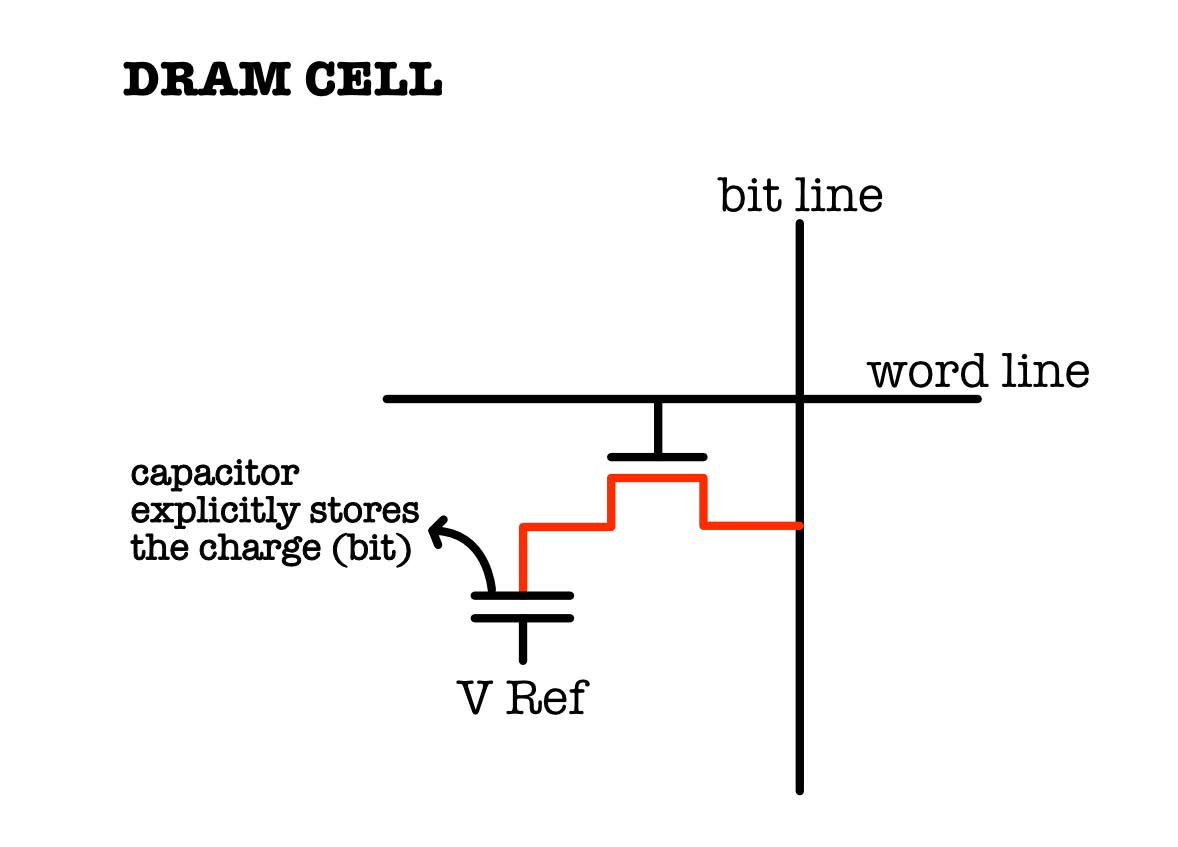
\includegraphics[width = 5.5cm]{DRAM_cell}
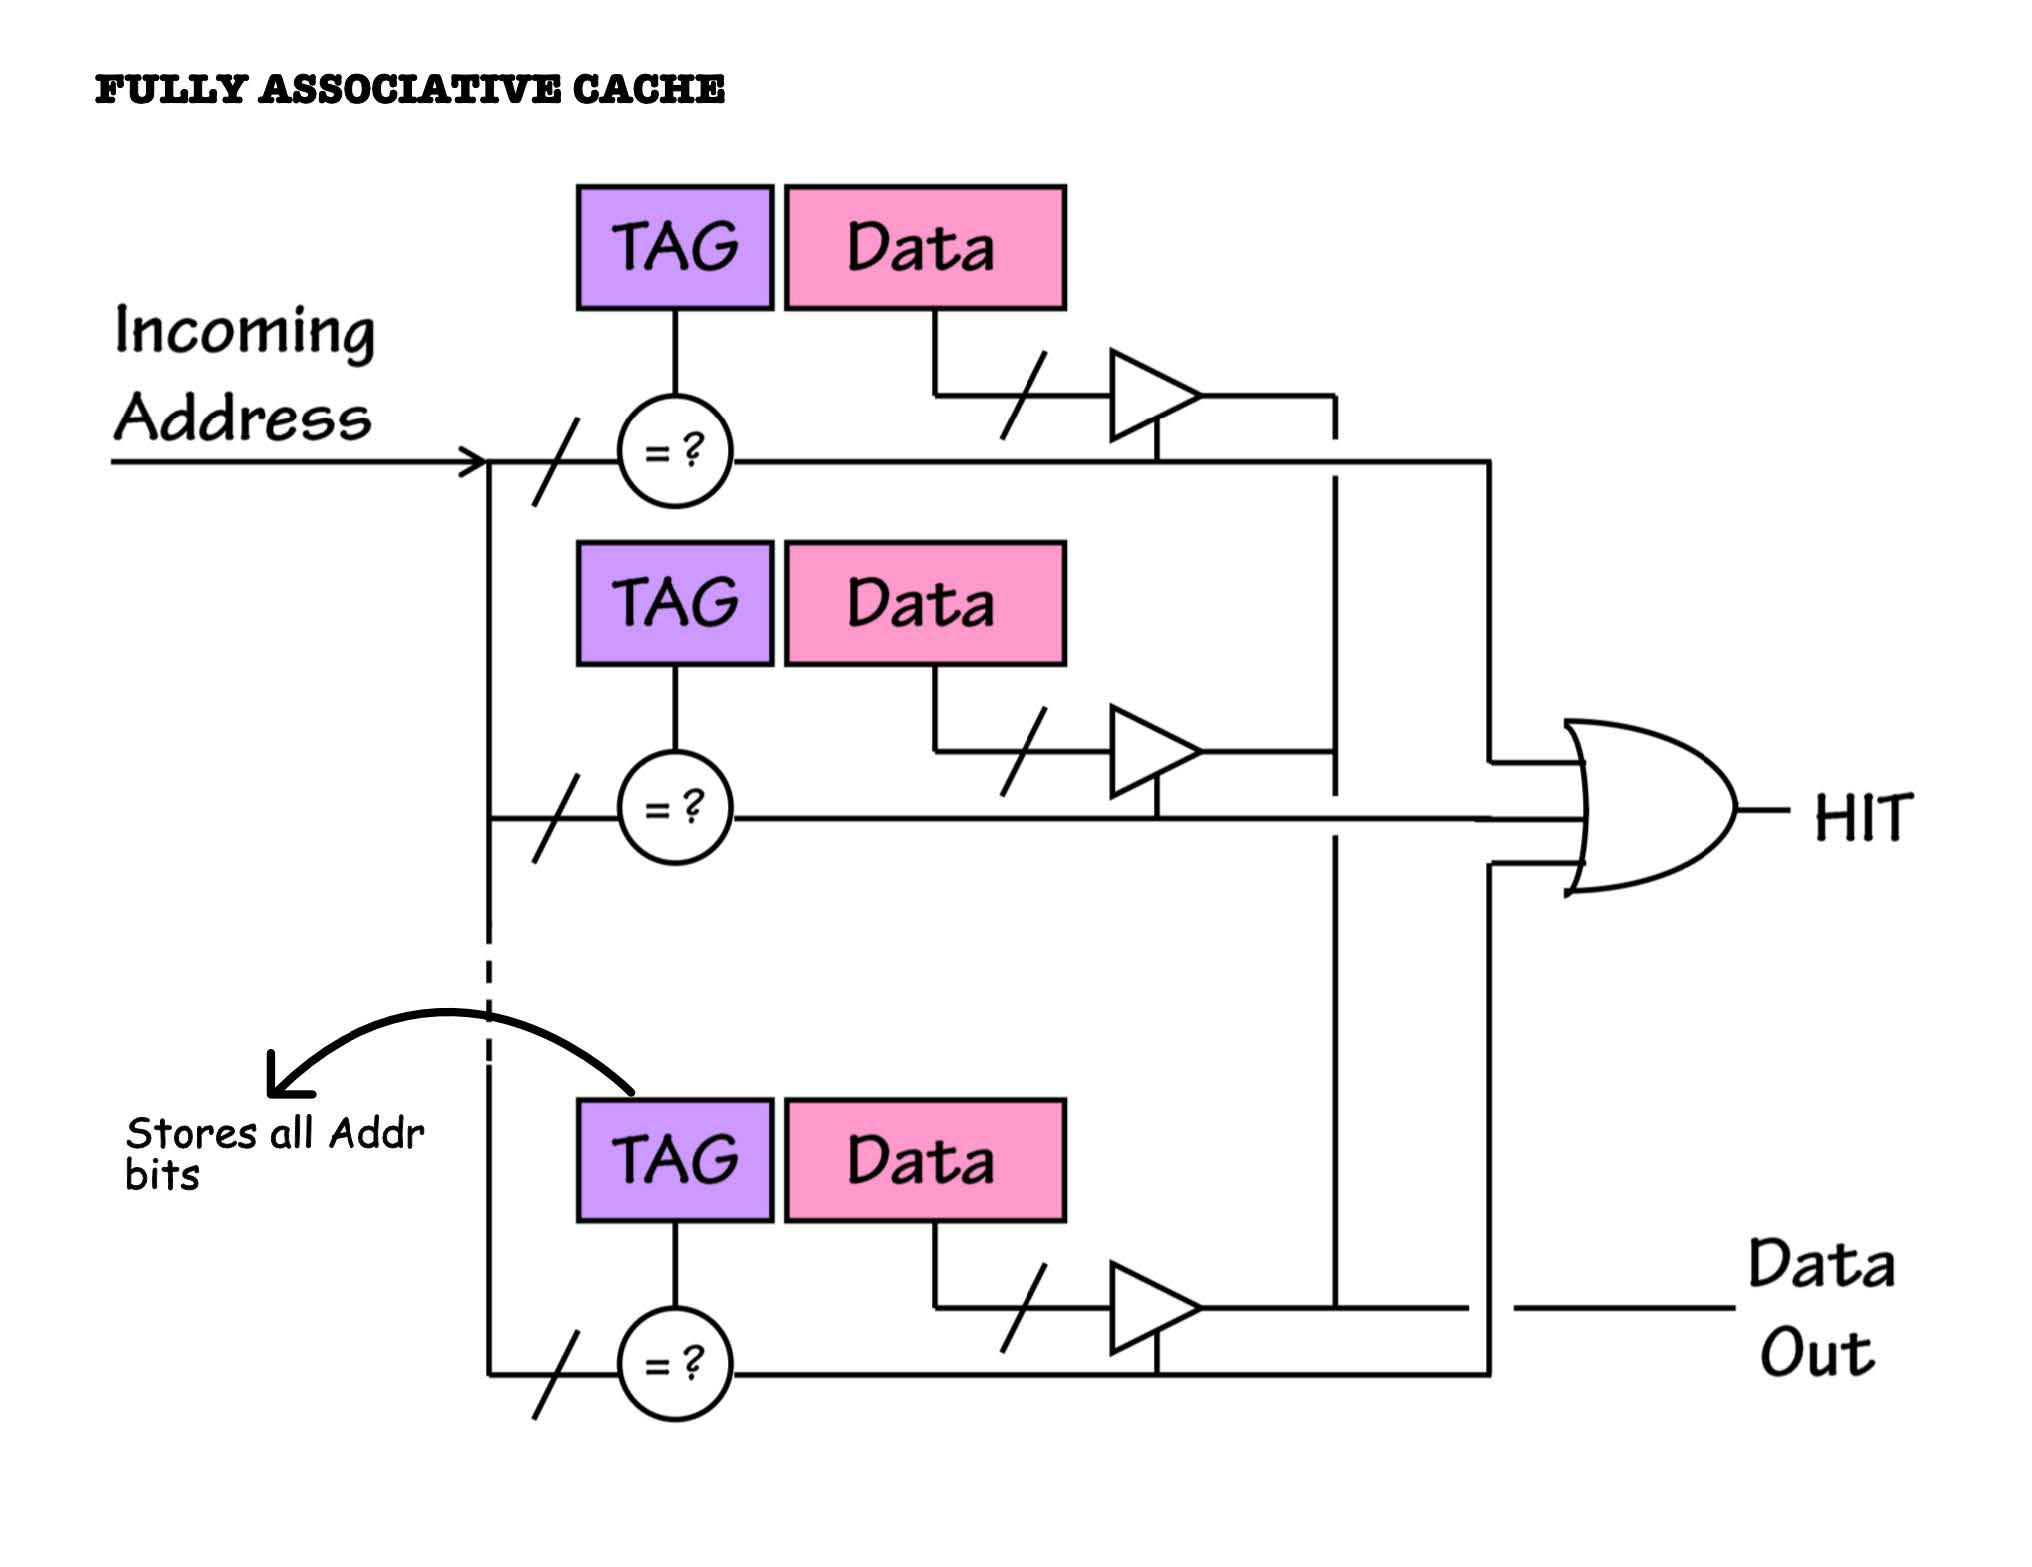
\includegraphics[width = 5.5cm]{FA_cache}
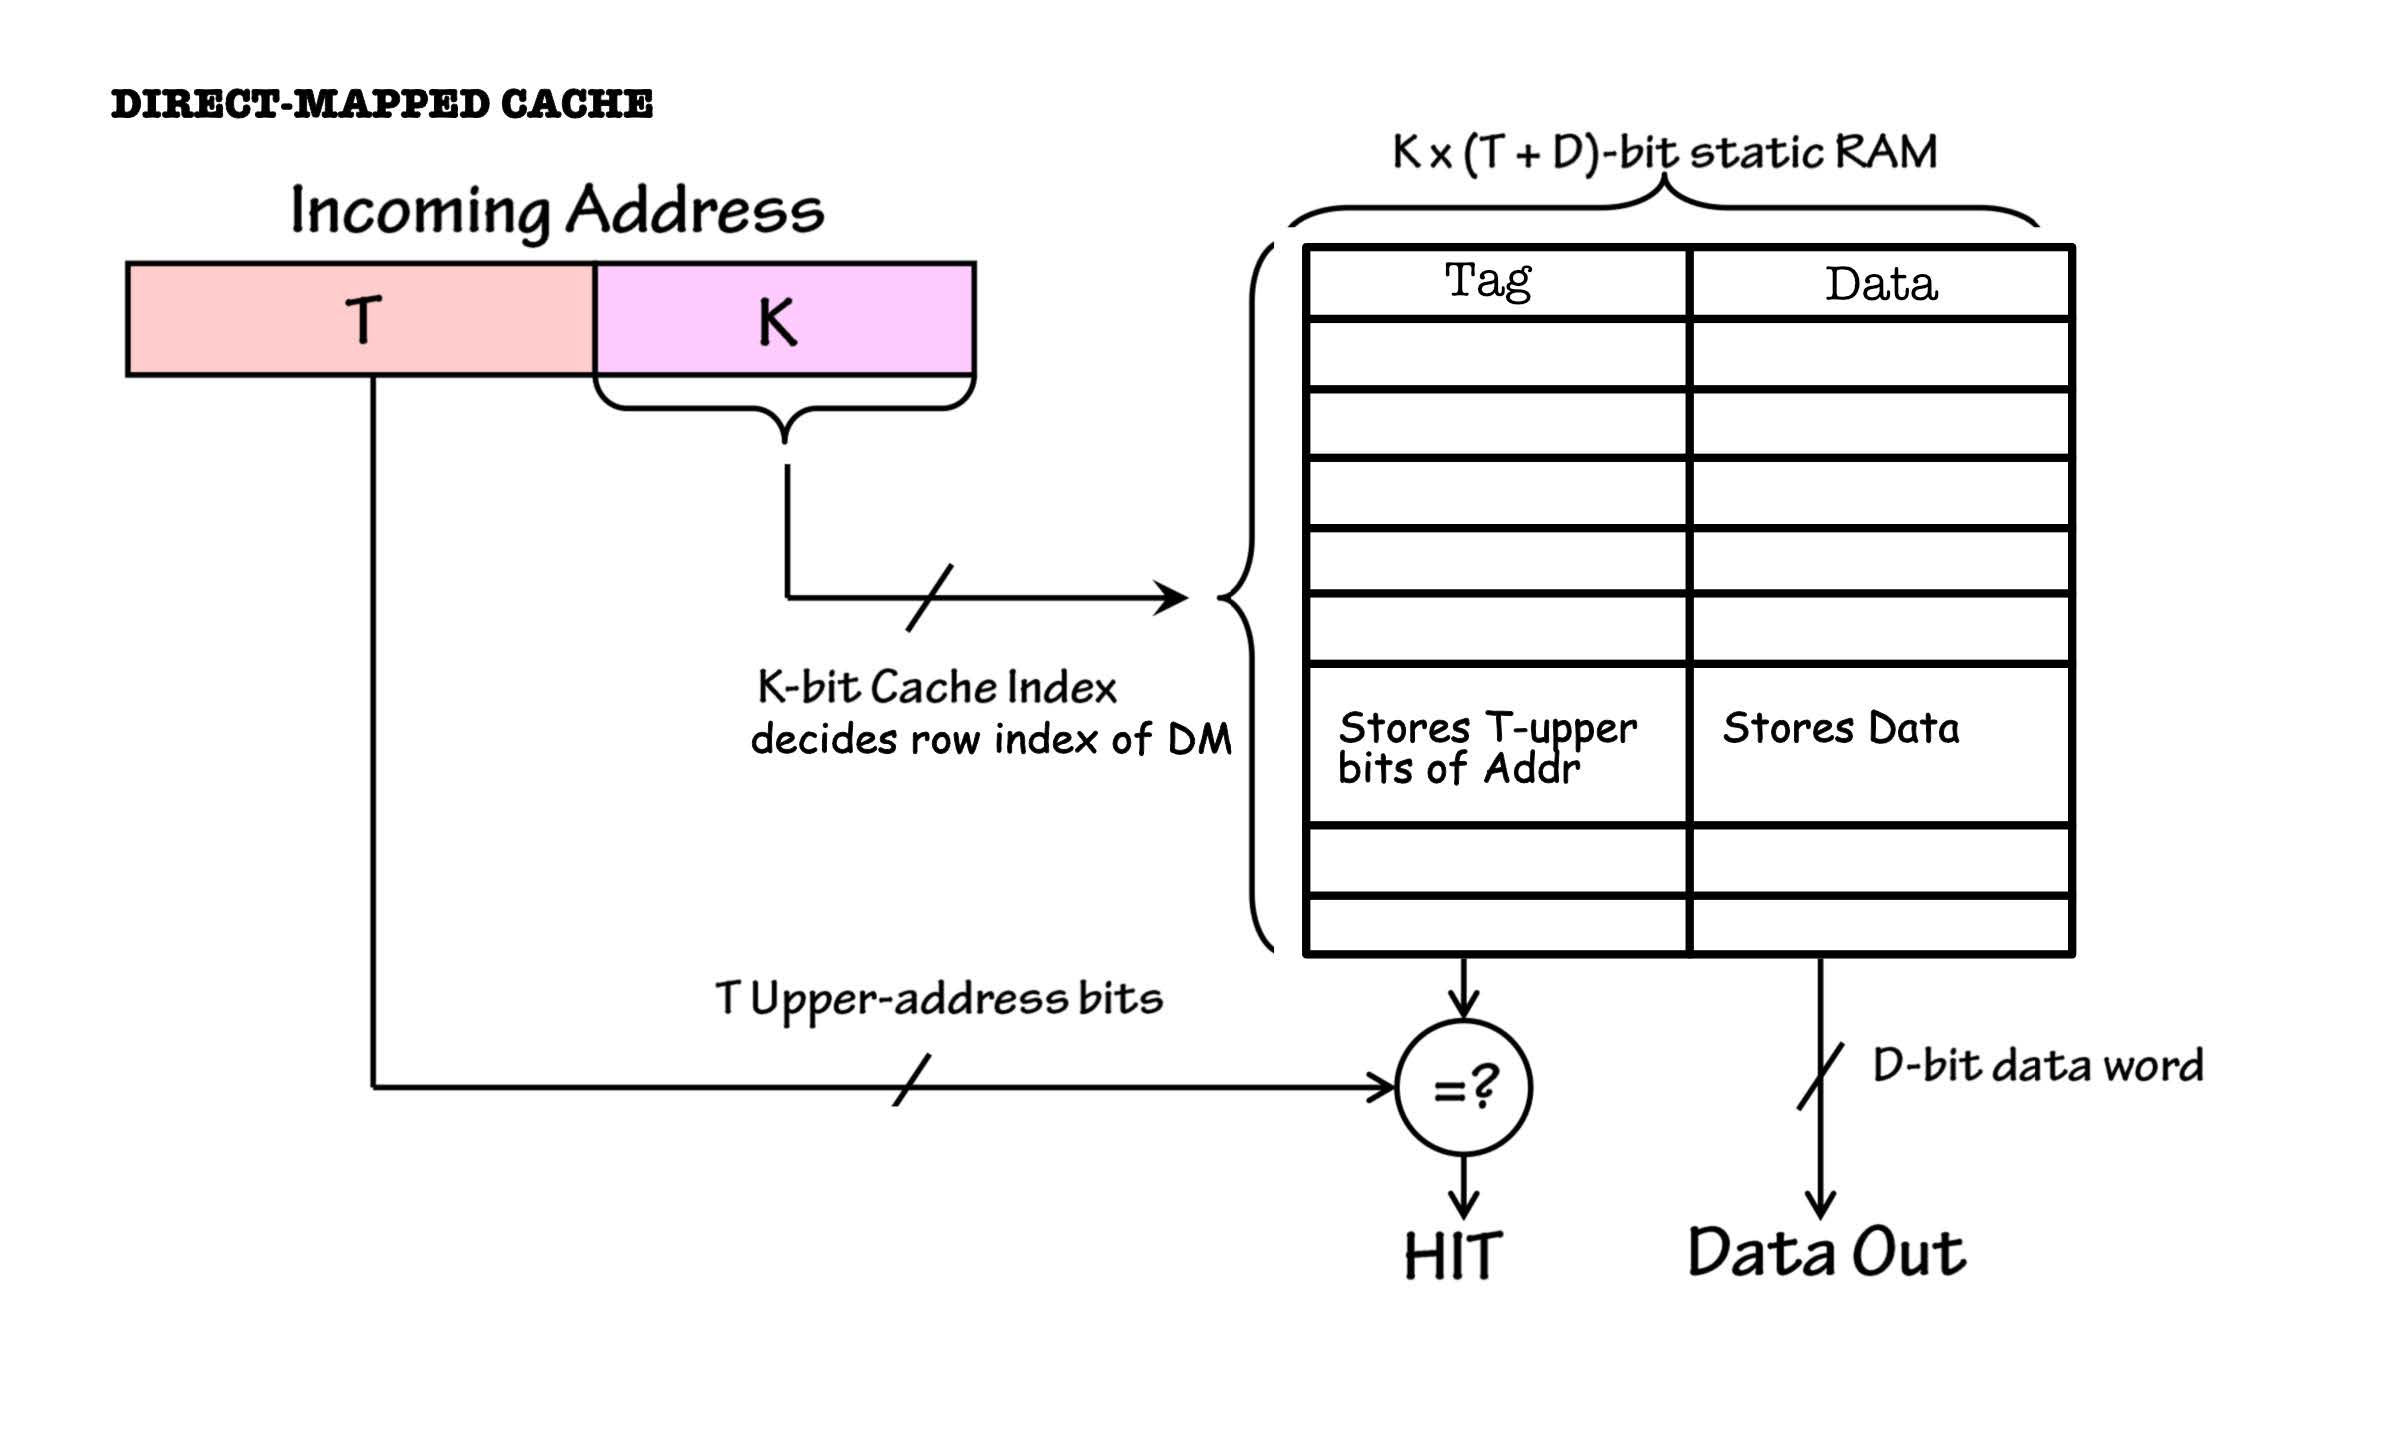
\includegraphics[width = 5.5cm]{DM_cache}
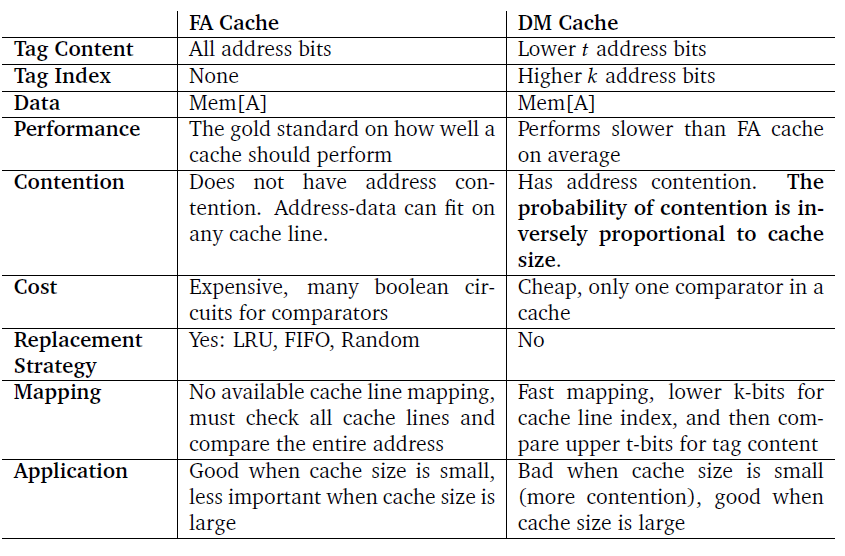
\includegraphics[width = 5.5cm]{cache_comparison}
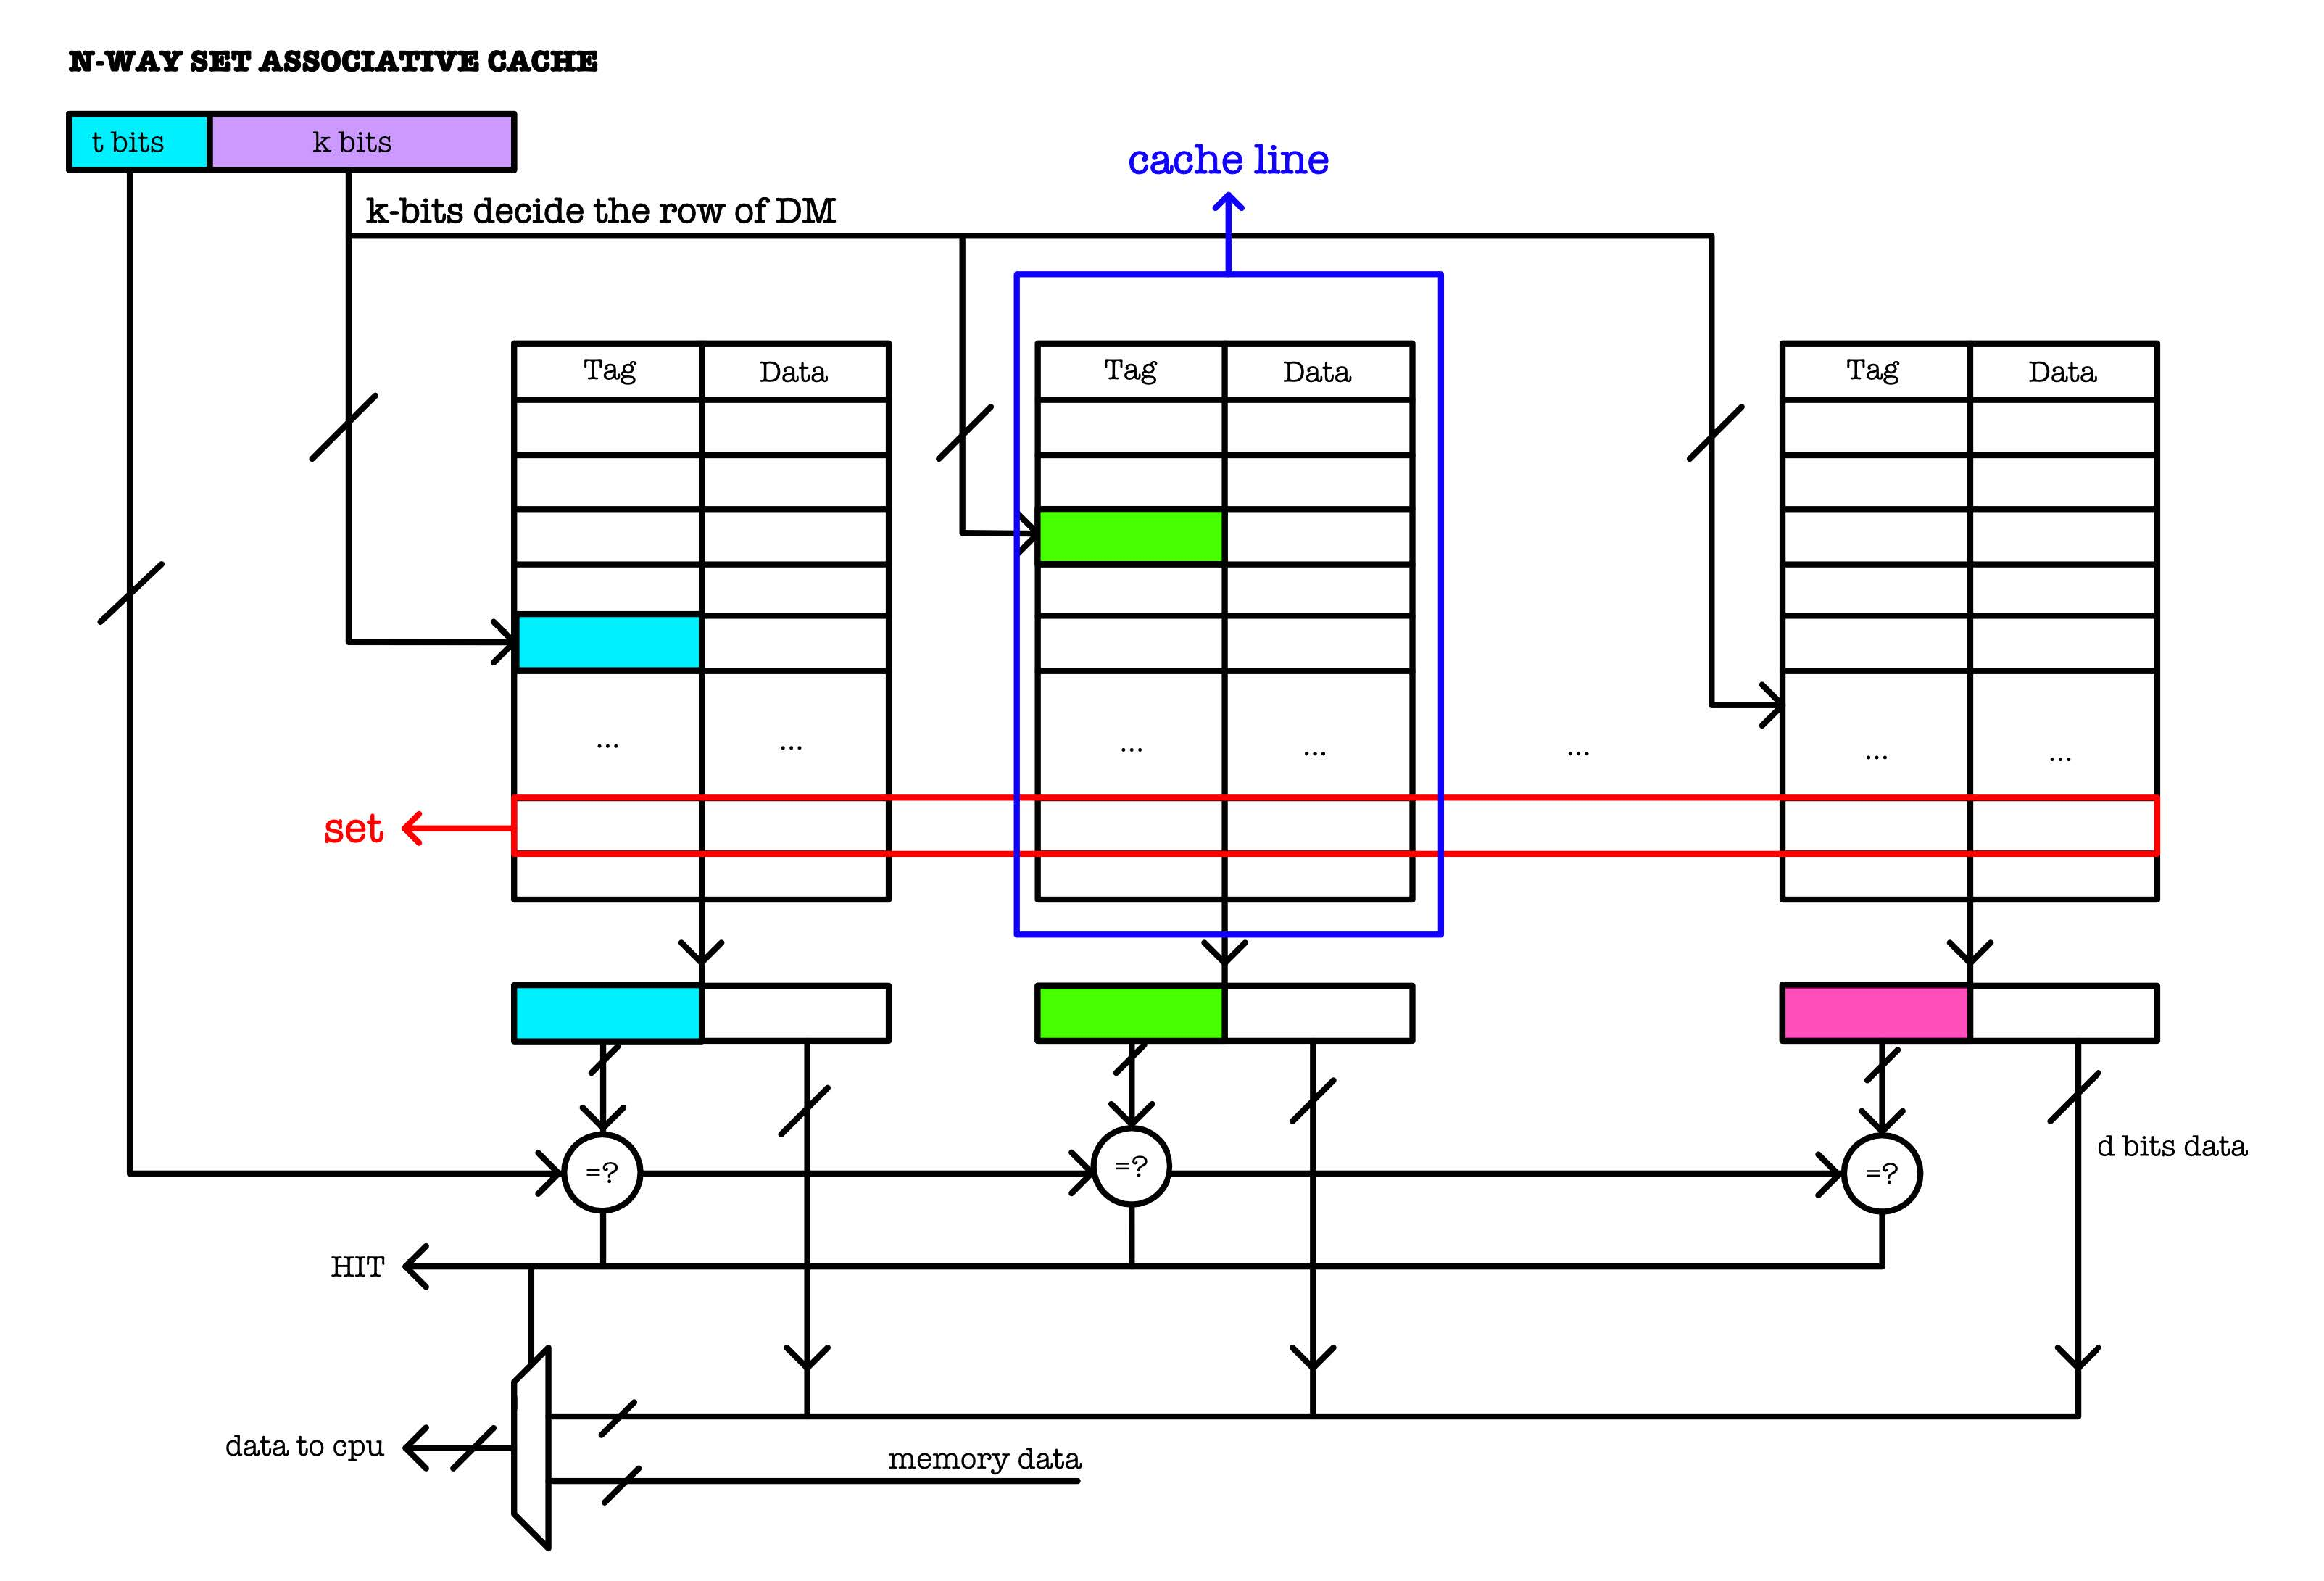
\includegraphics[width = 5.5cm]{N_way_cache}
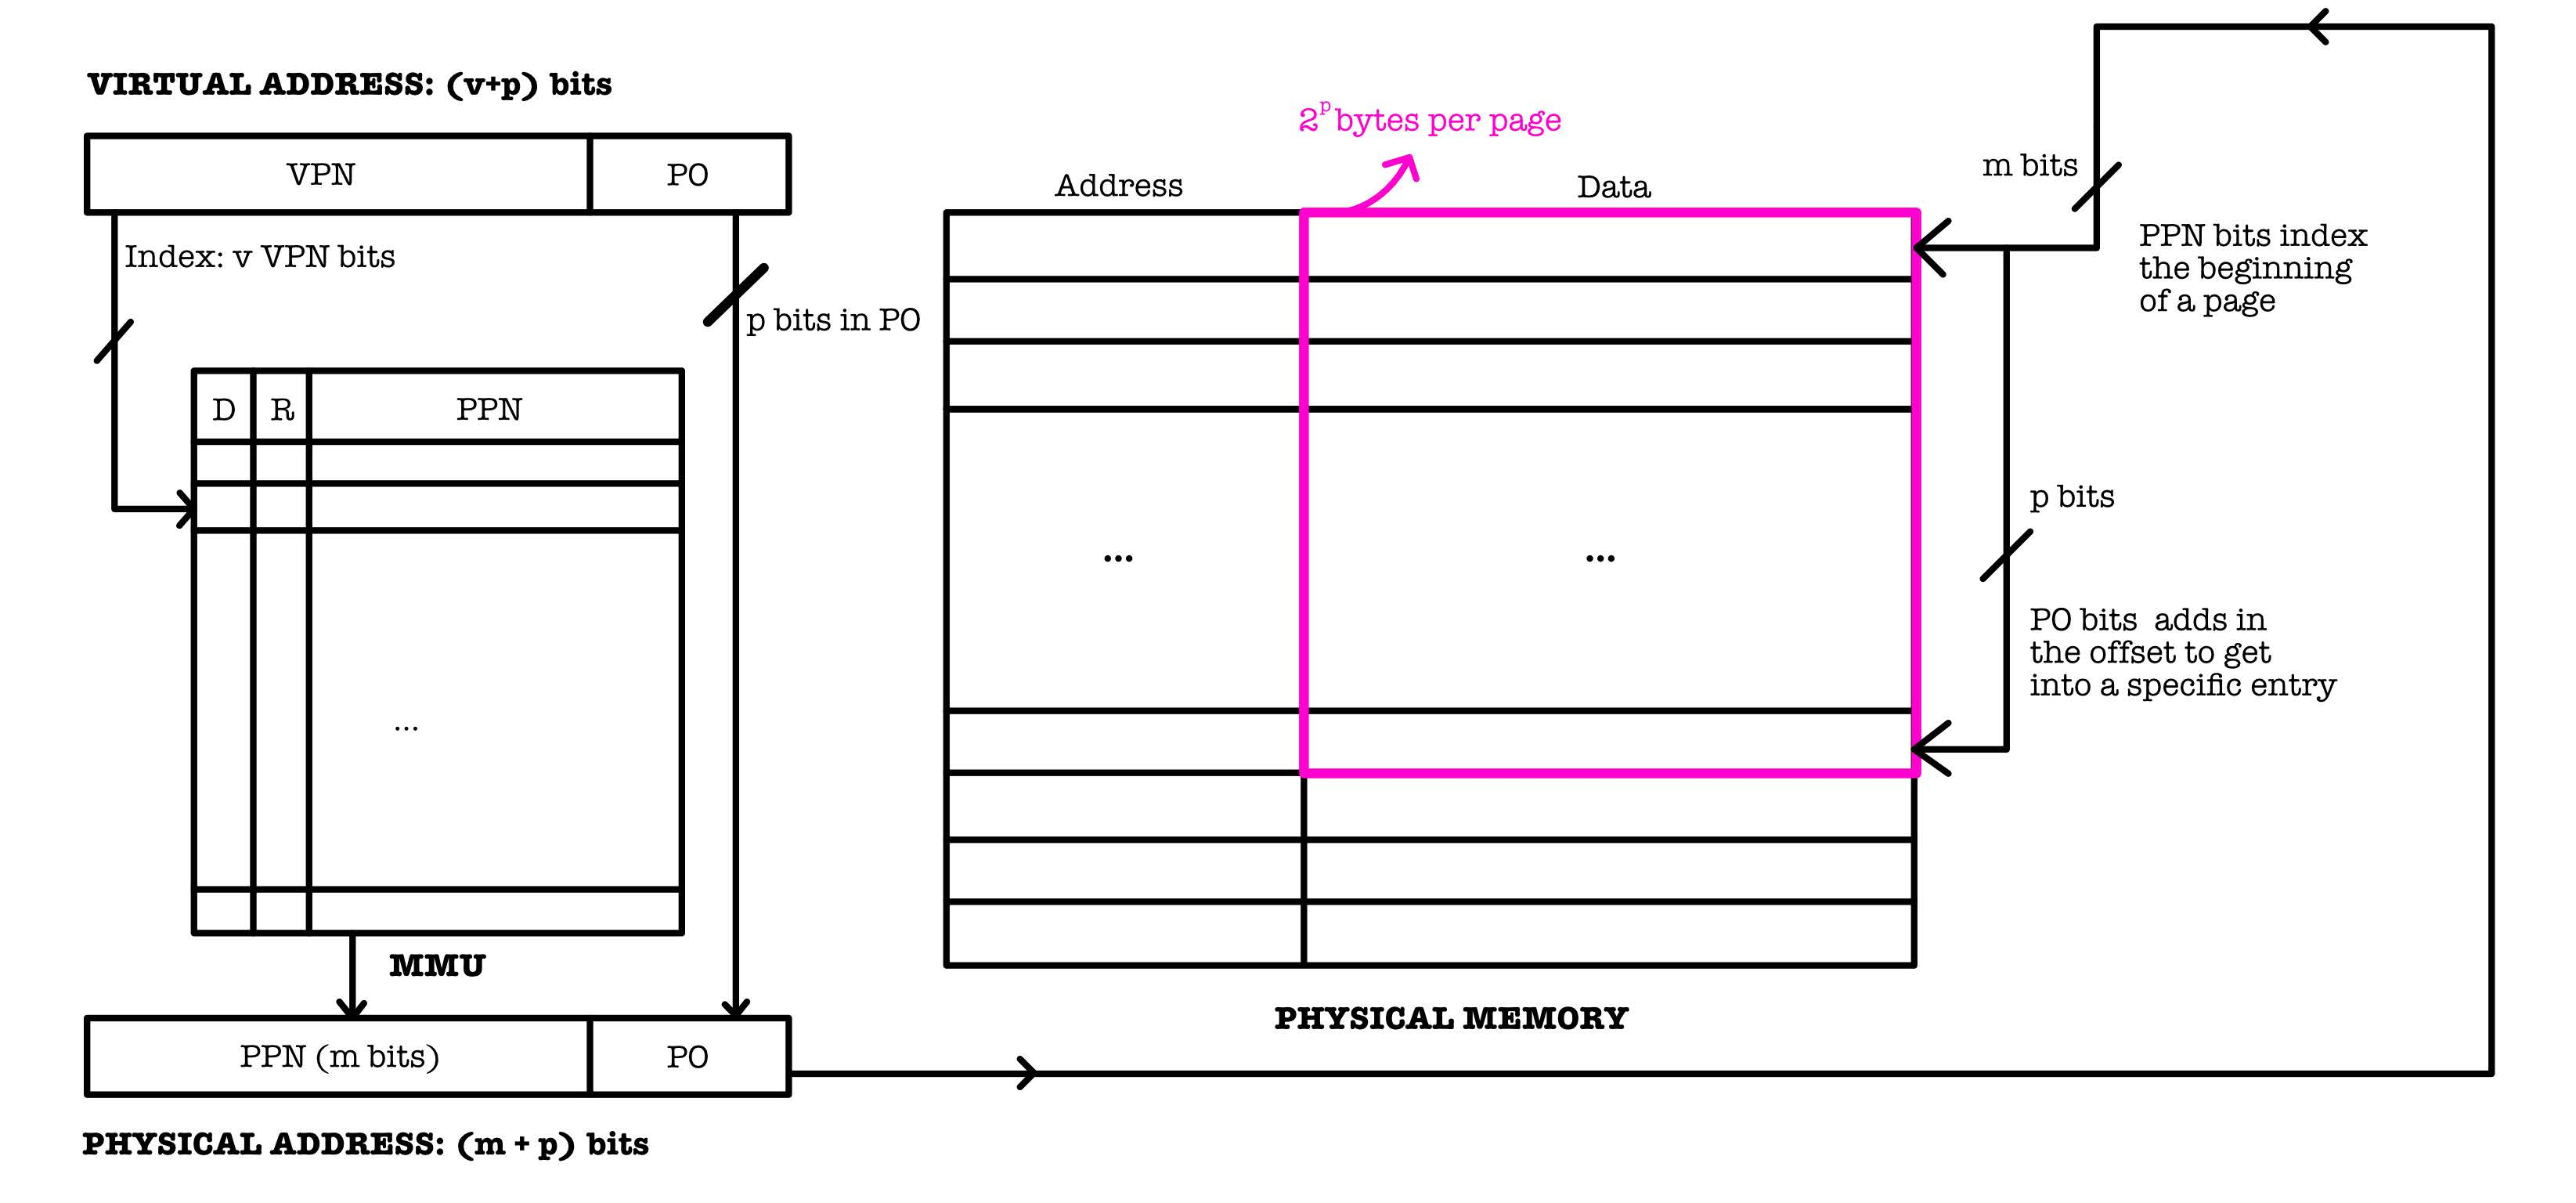
\includegraphics[width = 5.5cm]{Page_map}
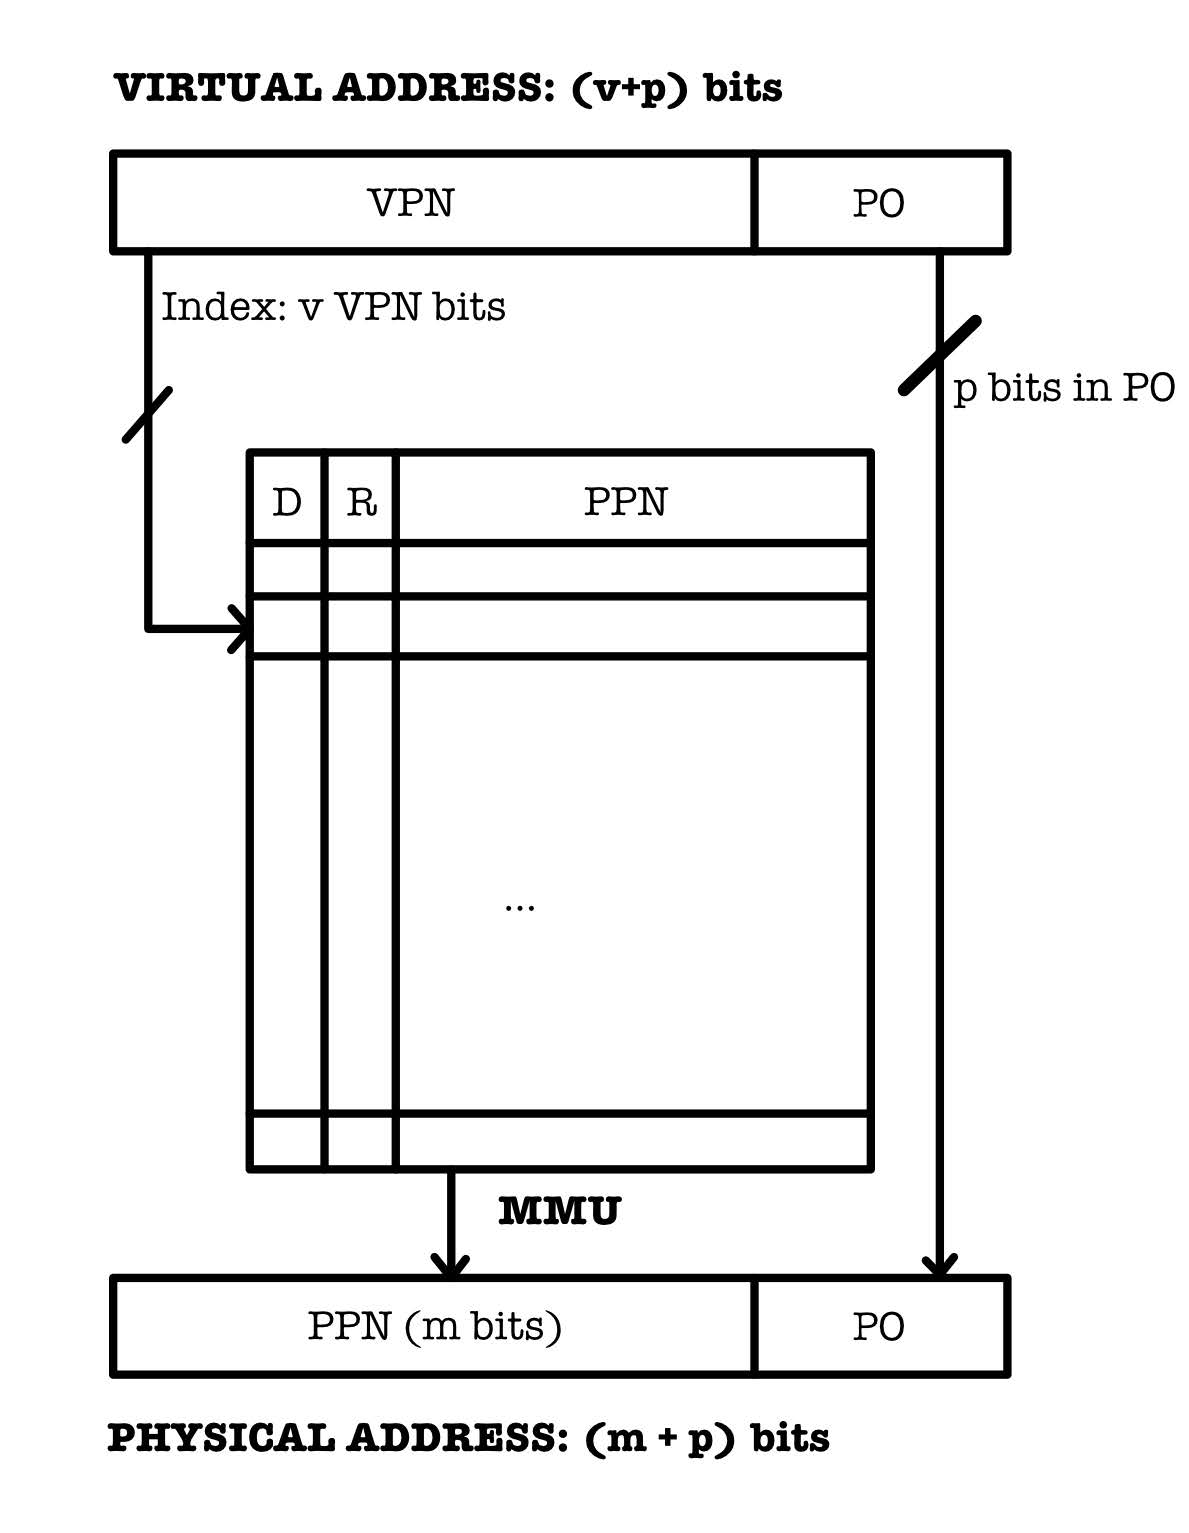
\includegraphics[width = 4.5cm]{MMU}
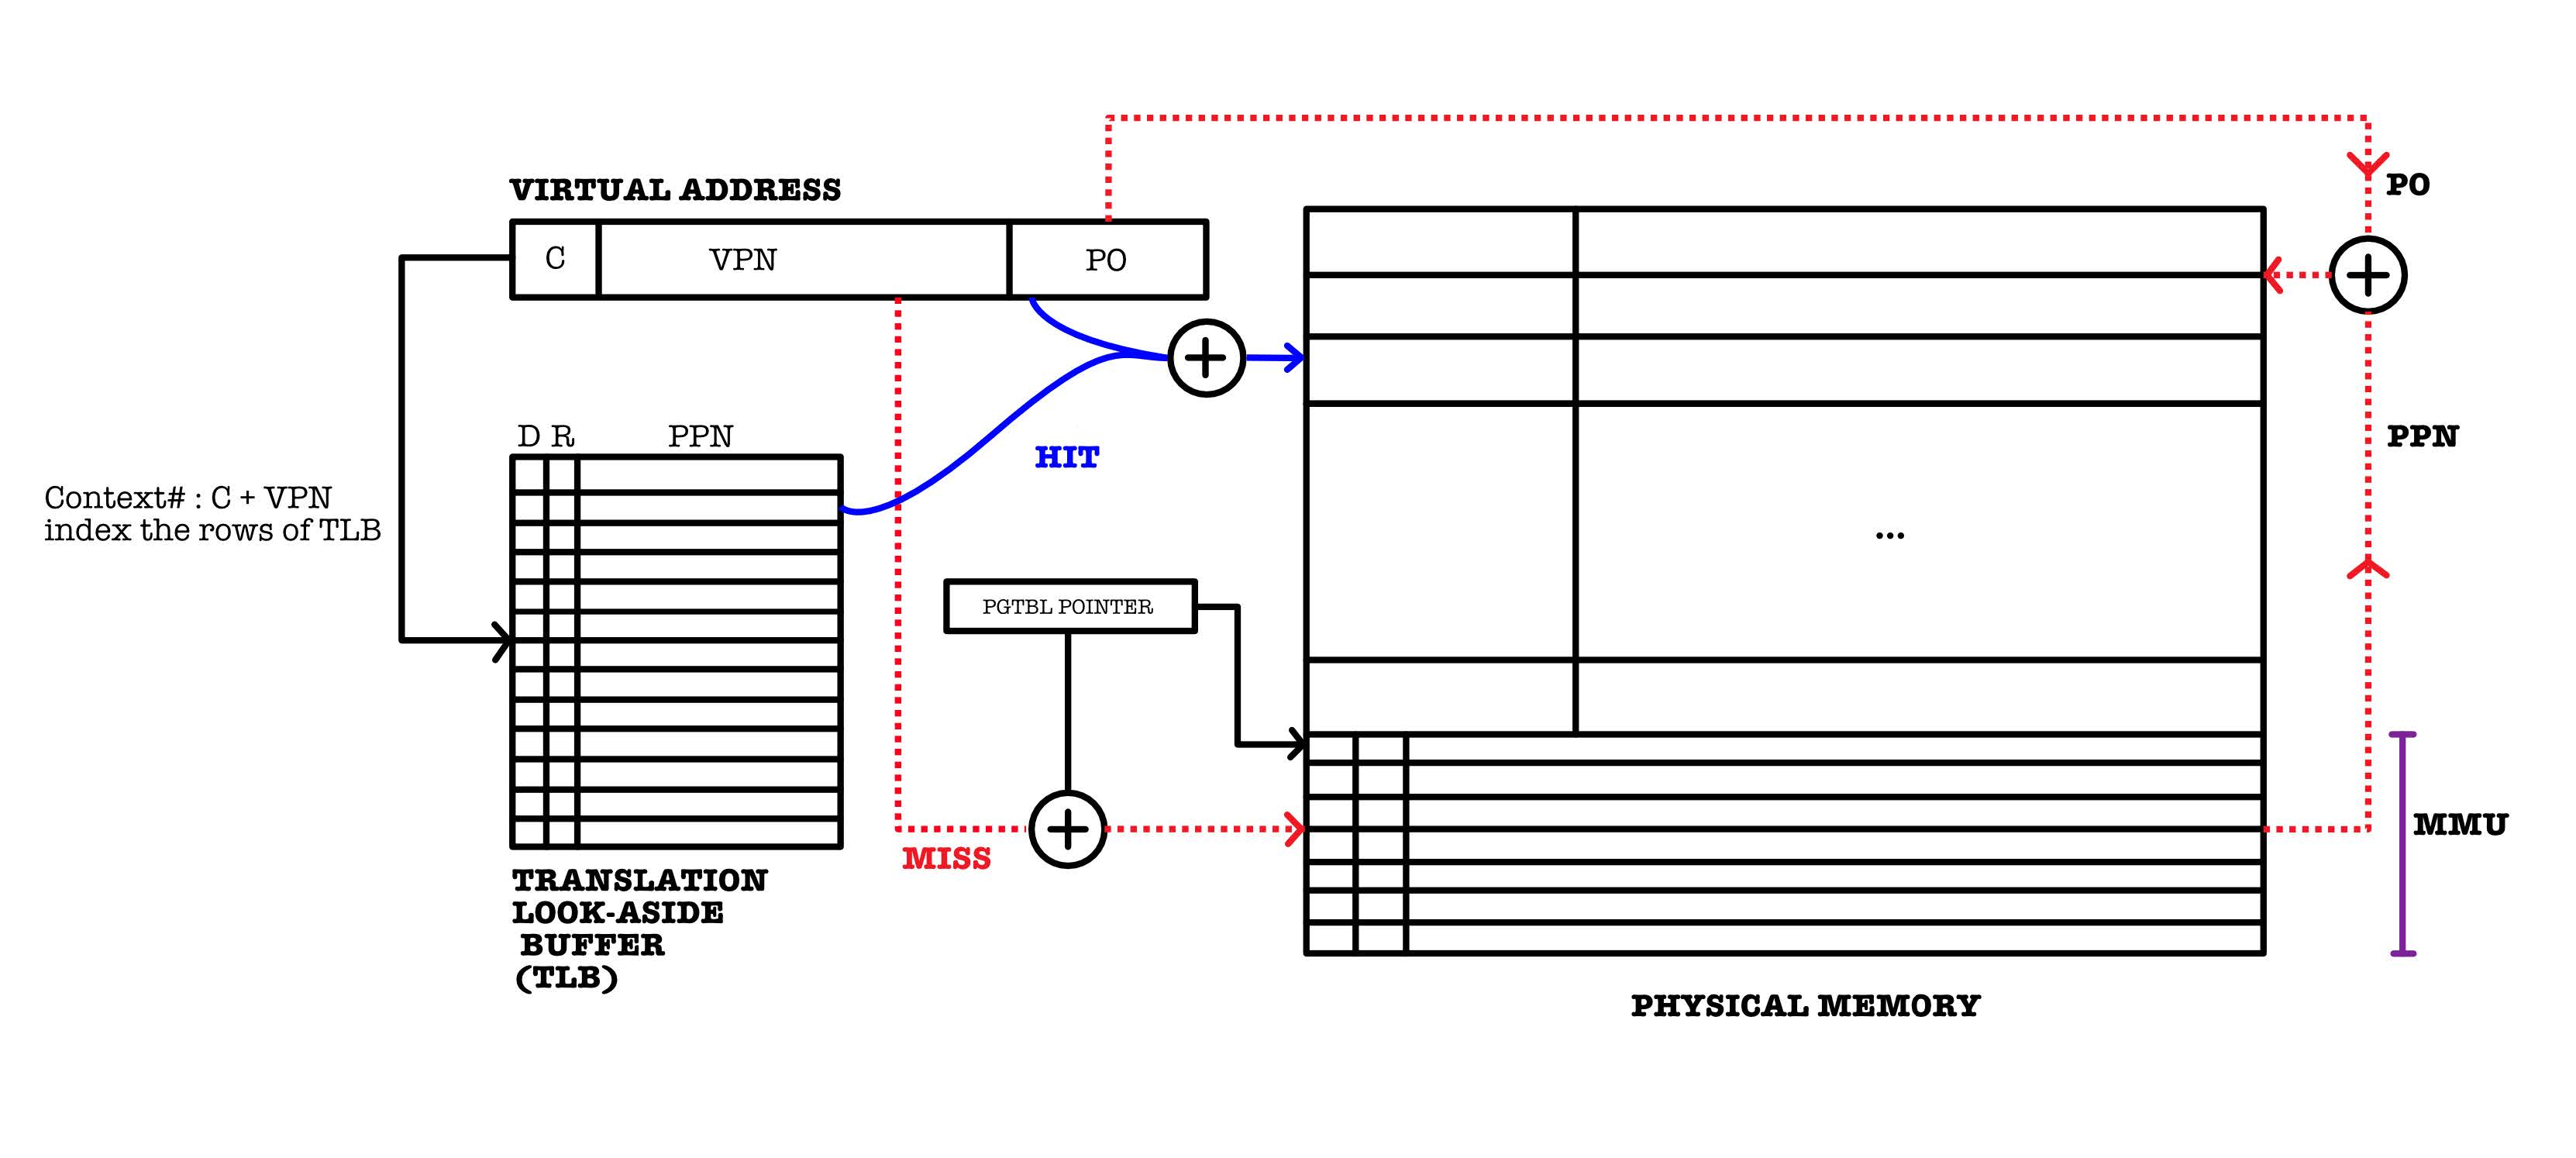
\includegraphics[width = 5.5cm]{TLB}
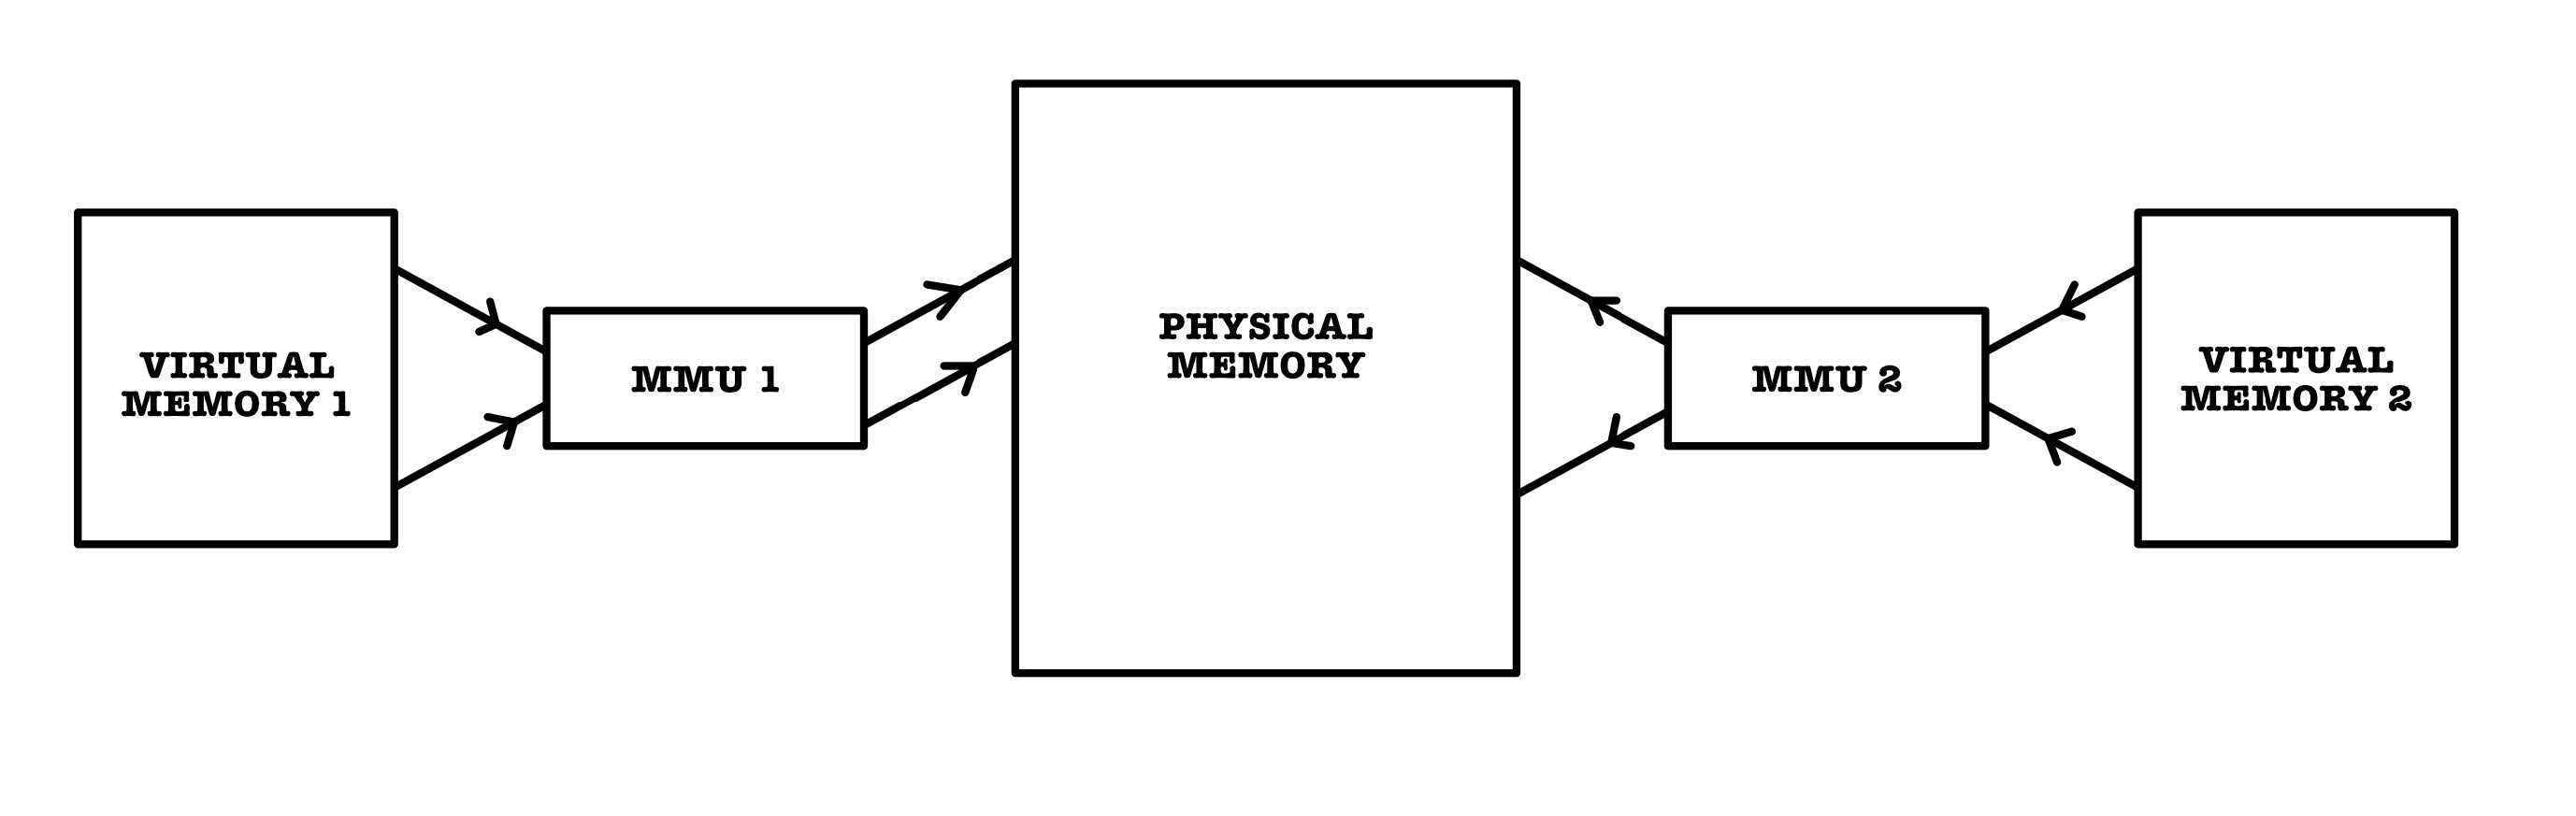
\includegraphics[width = 5.5cm]{Context}
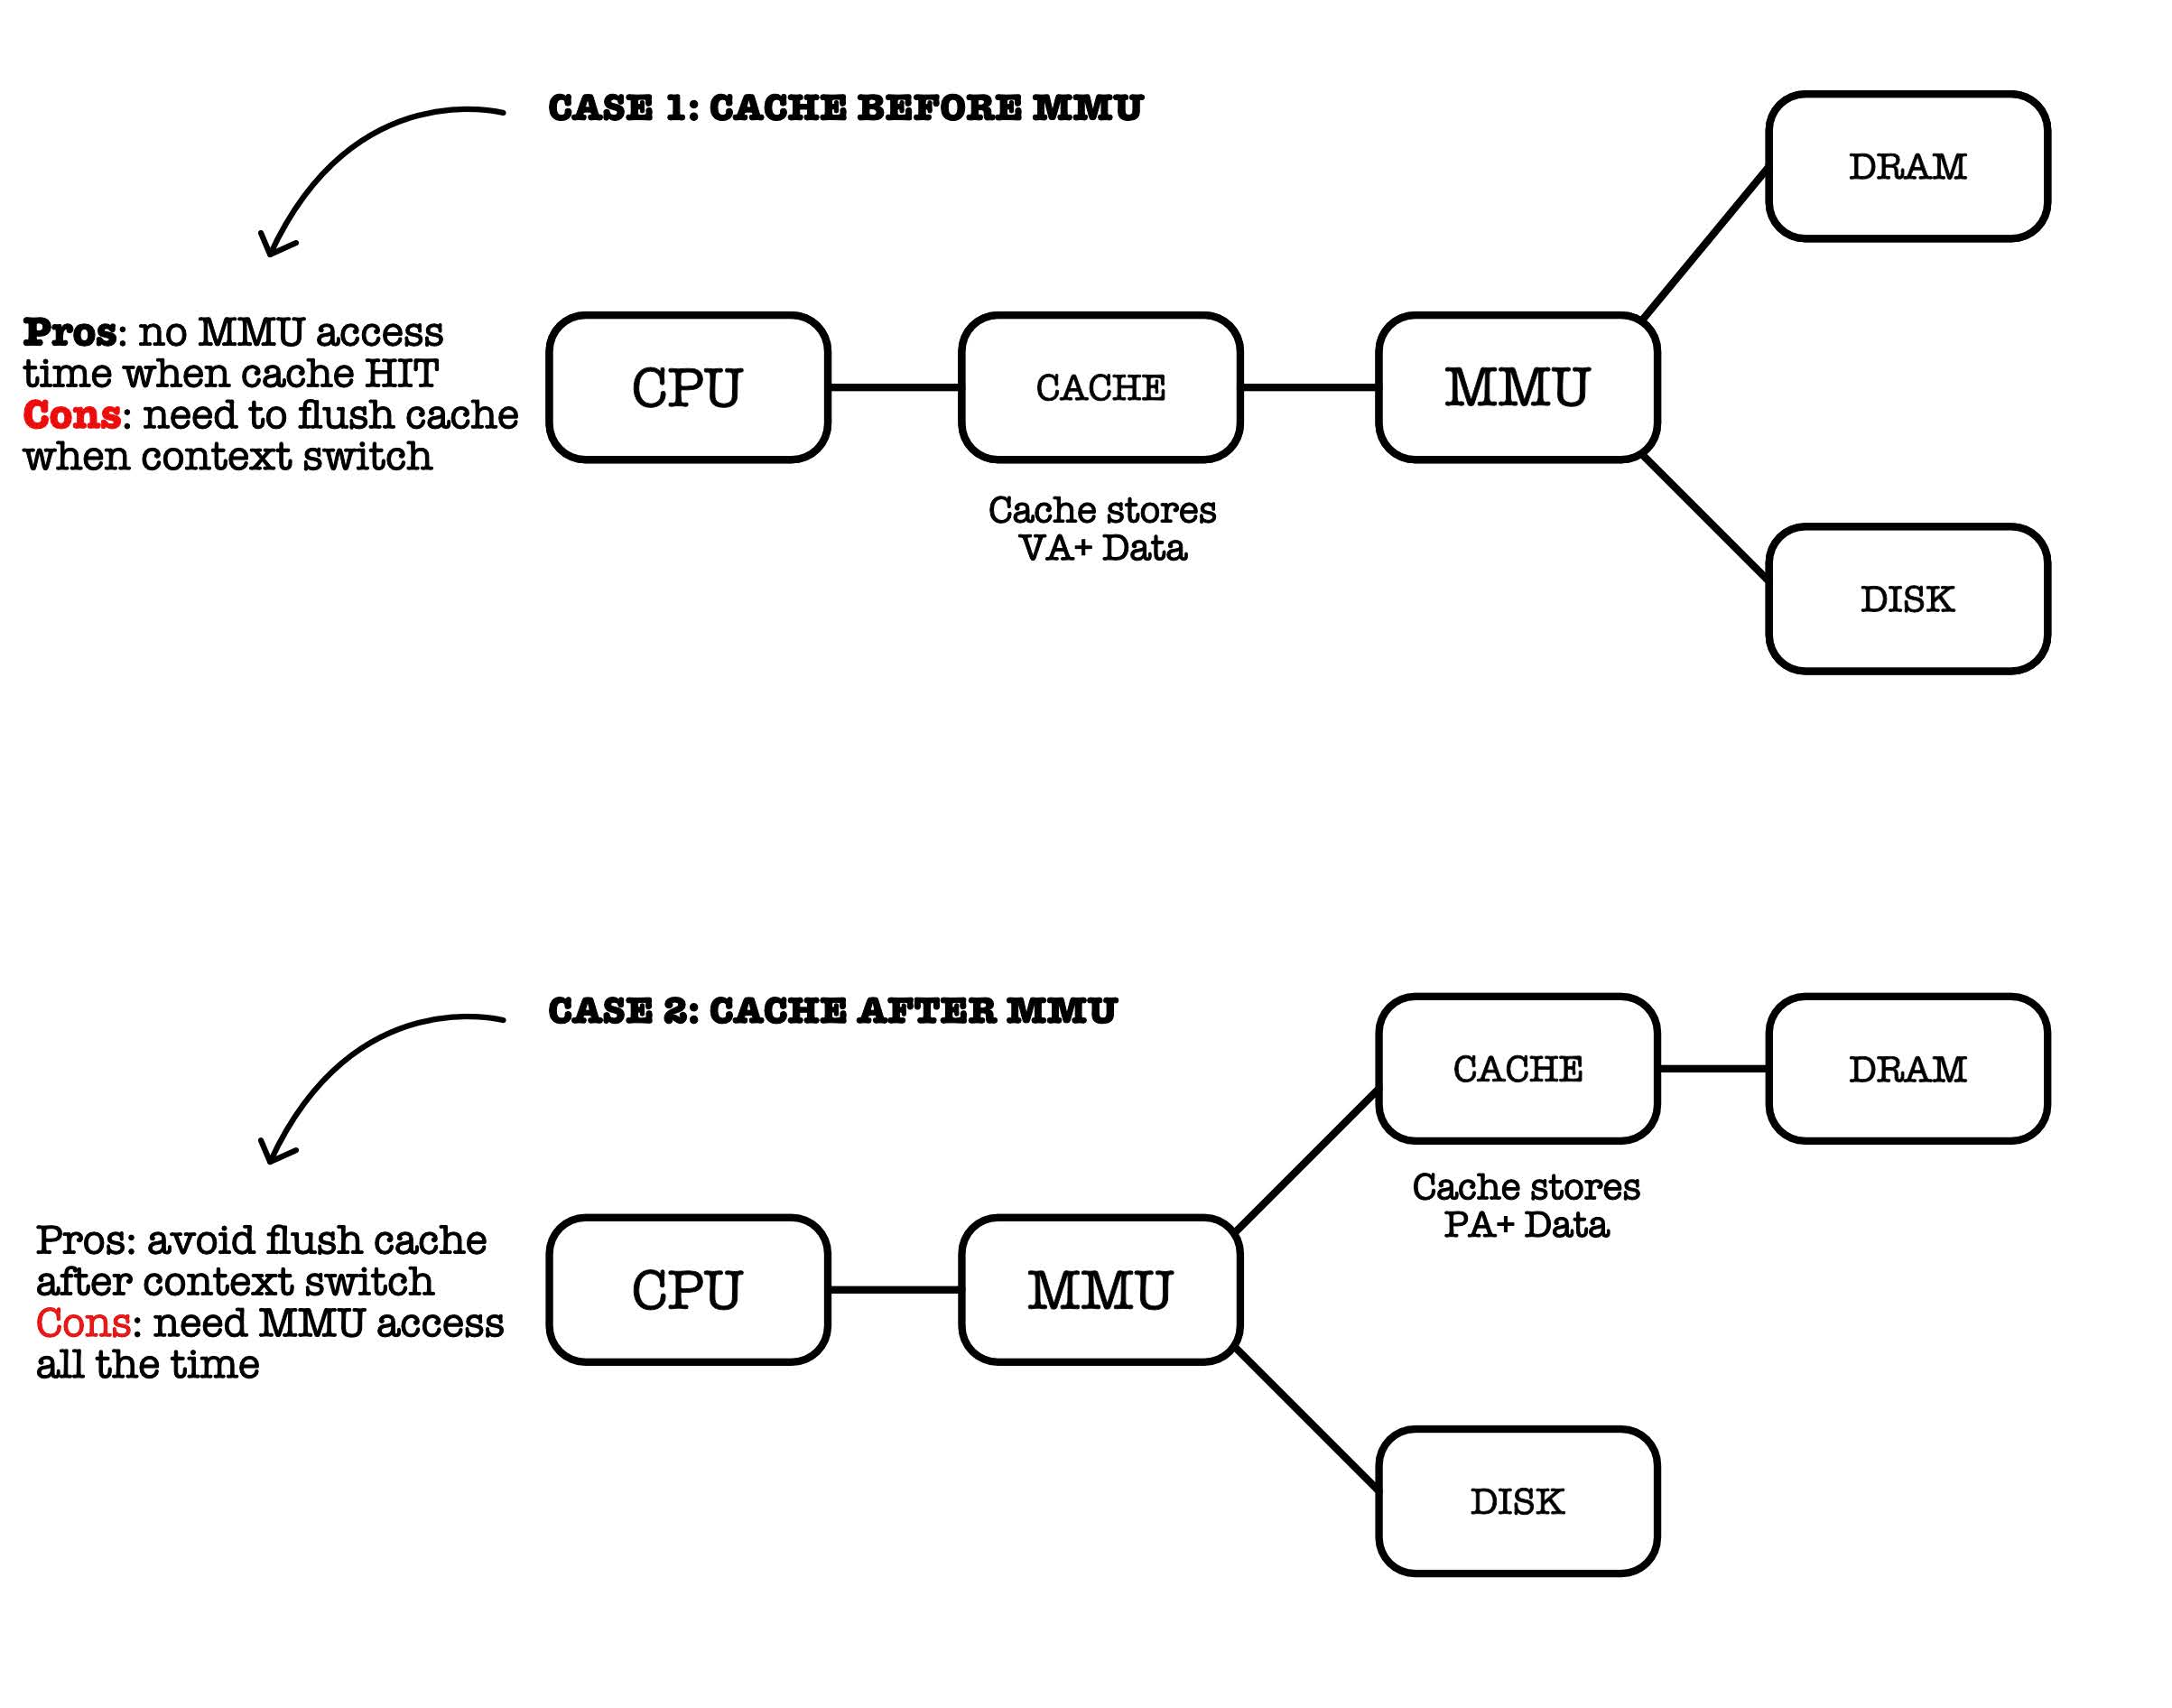
\includegraphics[width = 5.5cm]{VMCache}
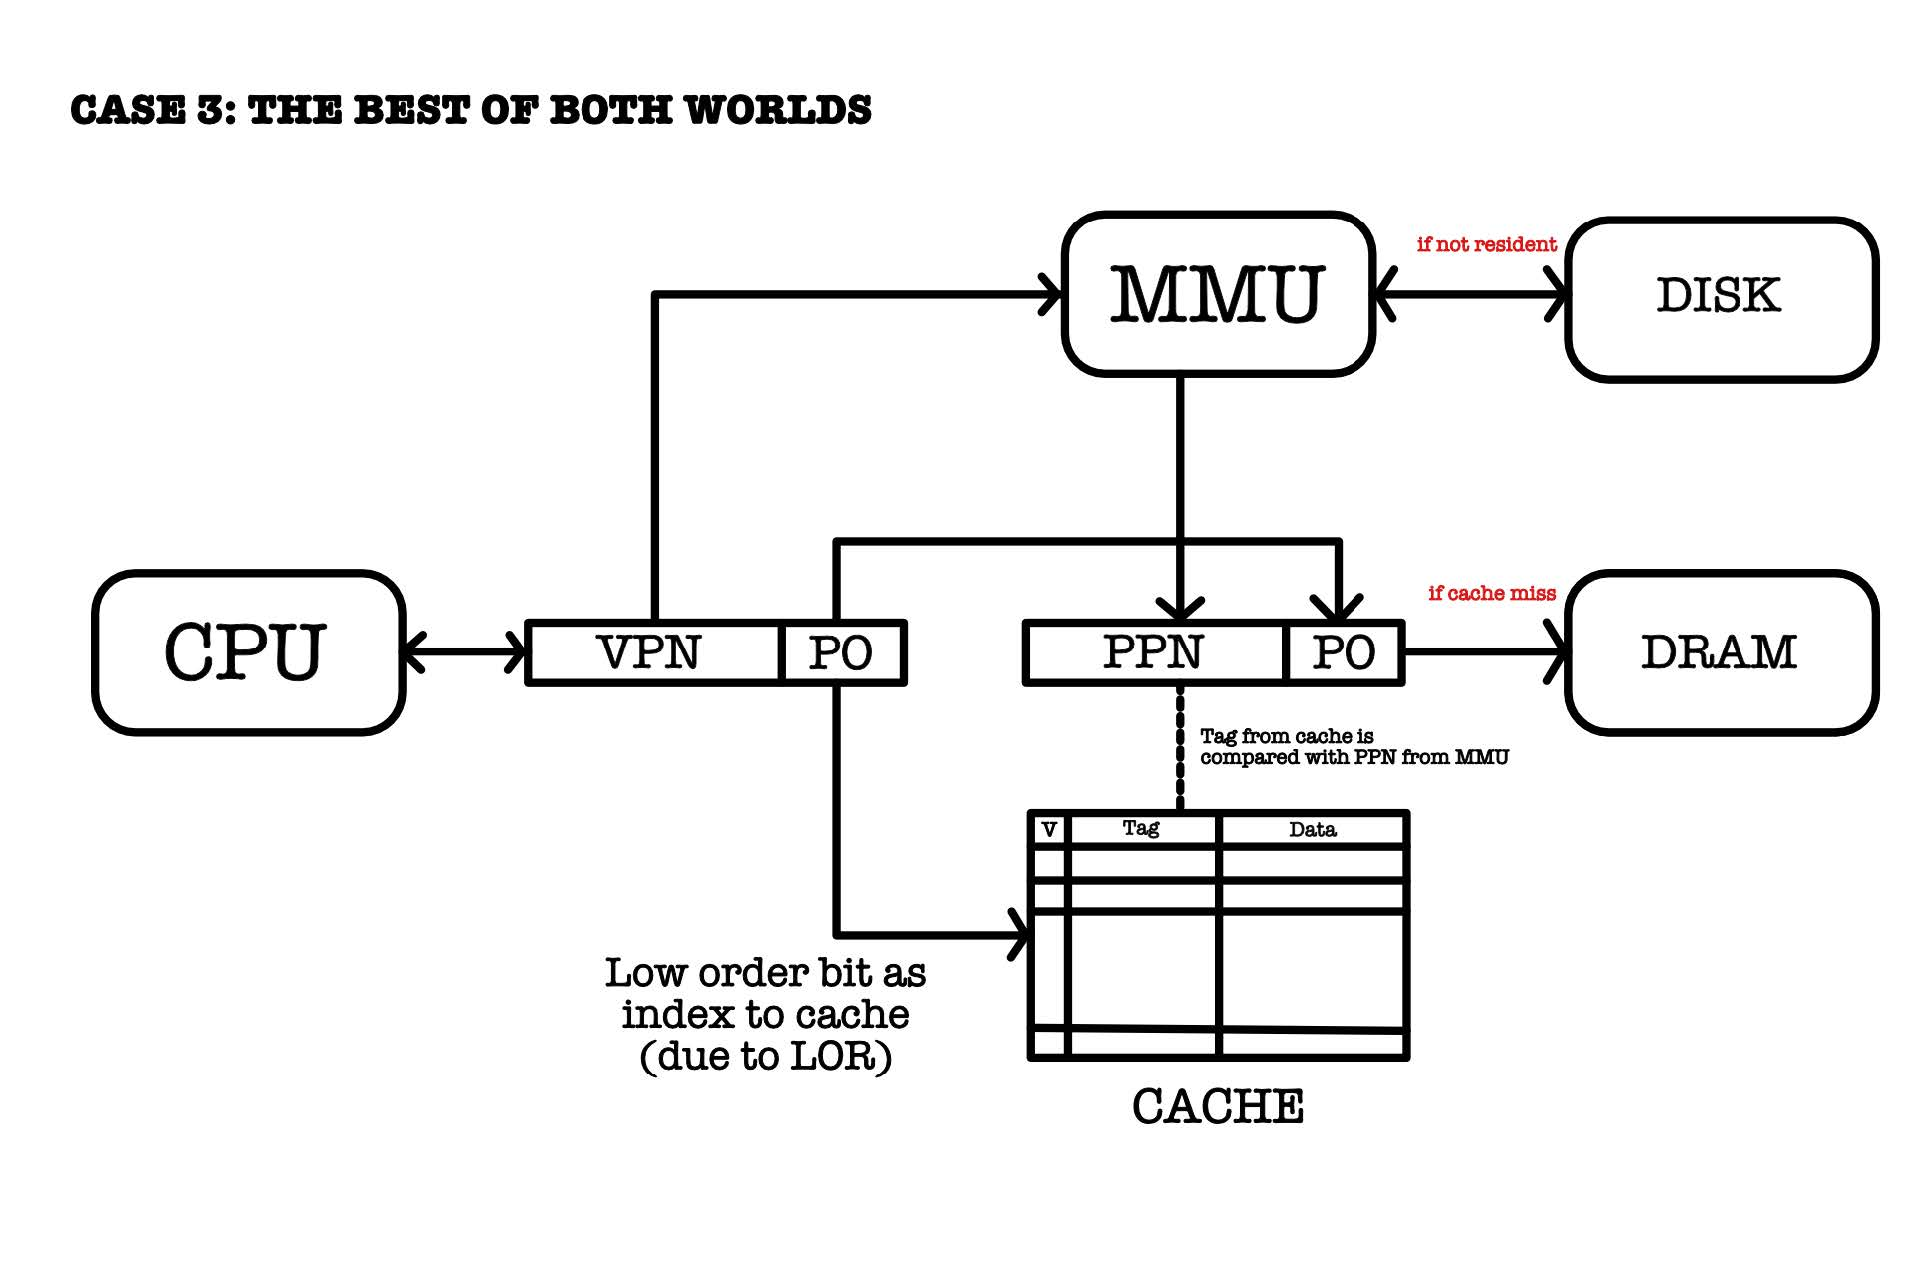
\includegraphics[width = 5.5cm]{VMBest}
\end{multicols*}
\end{document}